%%
%% This is file `sigplan.tex',
%% generated with the docstrip utility.
%%
%% The original source files were:
%%
%% samples.dtx  (with options: `all,proceedings,sigplan')
%% 
%% IMPORTANT NOTICE:
%% 
%% For the copyright see the source file.
%% 
%% Any modified versions of this file must be renamed
%% with new filenames distinct from sigplan.tex.
%% 
%% For distribution of the original source see the terms
%% for copying and modification in the file samples.dtx.
%% 
%% This generated file may be distributed as long as the
%% original source files, as listed above, are part of the
%% same distribution. (The sources need not necessarily be
%% in the same archive or directory.)
%%
%%
%% Commands for TeXCount
%TC:macro \cite [option:text,text]
%TC:macro \citep [option:text,text]
%TC:macro \citet [option:text,text]
%TC:envir table 0 1
%TC:envir table* 0 1
%TC:envir tabular [ignore] word
%TC:envir displaymath 0 word
%TC:envir math 0 word
%TC:envir comment 0 0
%%
%% The first command in your LaTeX source must be the \documentclass
%% command.
%%
%% For submission and review of your manuscript please change the
%% command to \documentclass[manuscript, screen, review]{acmart}.
%%
%% When submitting camera ready or to TAPS, please change the command
%% to \documentclass[sigconf]{acmart} or whichever template is required
%% for your publication.
%%
%%
% \documentclass[sigplan,screen,review,anonymous]{acmart}
\documentclass[sigplan,screen,review]{acmart}
% \documentclass[sigplan,screen,review,anonymous]{acmart}

%%
%% \BibTeX command to typeset BibTeX logo in the docs
\AtBeginDocument{%
  \providecommand\BibTeX{{%
    Bib\TeX}}}

% arxiv
\setcopyright{none}
\copyrightyear{2027}
\acmYear{2027}
\acmDOI{XXXXXXX.XXXXXXX}
\acmConference[Accepted (shepherding) to CGO'27]{Accepted (shepherding) to CGO'27}{USA}{2027}
\acmISBN{978-1-4503-XXXX-X/2018/06}
% ACMRef: Set to false for initial submission/arxiv
\settopmatter{printacmref=false}
\setcopyright{none}
\settopmatter{printacmref=false}
\renewcommand\footnotetextcopyrightpermission[1]{}

%%
%% Submission ID.
%% Use this when submitting an article to a sponsored event. You'll
%% receive a unique submission ID from the organizers
%% of the event, and this ID should be used as the parameter to this command.
%%\acmSubmissionID{123-A56-BU3}

%%
%% For managing citations, it is recommended to use bibliography
%% files in BibTeX format.
%%
%% You can then either use BibTeX with the ACM-Reference-Format style,
%% or BibLaTeX with the acmnumeric or acmauthoryear sytles, that include
%% support for advanced citation of software artefact from the
%% biblatex-software package, also separately available on CTAN.
%%
%% Look at the sample-*-biblatex.tex files for templates showcasing
%% the biblatex styles.
%%
%%
%% The majority of ACM publications use numbered citations and
%% references.  The command \citestyle{authoryear} switches to the
%% "author year" style.
%%
%% If you are preparing content for an event
%% sponsored by ACM SIGGRAPH, you must use the "author year" style of
%% citations and references.
%% Uncommenting
%% the next command will enable that style.
%%\citestyle{acmauthoryear}


\usepackage{booktabs}
\usepackage{multirow}
\usepackage{tabularx}
\usepackage{array}
\usepackage{xcolor}
\usepackage{xspace}
\usepackage{svg} 

% Draft-only markers. Remove all \resultneeded entries before submission.
\definecolor{pendingred}{RGB}{165,28,48}
\newcommand{\systemname}{\textsc{QPU-XLA}\xspace}
\newcommand{\resultneeded}[1]{\textcolor{pendingred}{\textbf{[RESULT NEEDED: #1]}}}
\newcommand{\figplaceholder}[4]{%
  \begin{figure}[t]
    \centering
    \fbox{\parbox[c][#1][c]{0.93\columnwidth}{\centering\small #2}}
    \caption{#3}
    \label{#4}
  \end{figure}}
\newcommand{\widefigplaceholder}[4]{%
  \begin{figure*}[t]
    \centering
    \fbox{\parbox[c][#1][c]{0.95\textwidth}{\centering\small #2}}
    \caption{#3}
    \label{#4}
  \end{figure*}}


%%
%% end of the preamble, start of the body of the document source.
\begin{document}

%%
%% The "title" command has an optional parameter,
%% allowing the author to define a "short title" to be used in page headers.
\title[Practical: Native CPU--QPU AI Inference on Raspberry Pi 5]{Practical: Building and Evaluating a Native CPU–QPU Runtime for Edge AI Inference on Raspberry Pi 5}

\author{Yiannis Hadjiyianni}
\authornote{Equal Contribution}
\email{yiannisha@synkrasis-labs.com}
\orcid{0009-0003-2413-6375}
\affiliation{%
  \institution{National Technical University of Athens}
  \city{Athens}
  \state{Attica}
  \country{Greece}
}


\author{Kun Ouyang}
% \authornotemark[1]
\email{kunouyang@stu.hit.edu.cn}
\orcid{0009-0006-4754-9625}
\affiliation{%
  \department{Faculty of Computing}
  \institution{Harbin Institute of Technology}
  \city{Harbin}
  \country{China}
}
% \affiliation{%
%   \institution{State Key Laboratory of Smart Farm Technologies and Systems}
%   \city{Harbin}
%   \country{China}
% }


\author{Linyuan Han}
% \authornotemark[1]
\email{linyuanhan26@stu.hit.edu.cn}
\orcid{0009-0009-2041-7202}
\affiliation{%
  \department{Faculty of Computing}
  \institution{Harbin Institute of Technology}
  \city{Harbin}
  \country{China}
}
% \affiliation{%
%   \institution{State Key Laboratory of Smart Farm Technologies and Systems}
%   \city{Harbin}
%   \country{China}
% }


\author{Panagiotis Michelakis}
\email{panosg@synkrasis-labs.com}
\orcid{0009-0003-0498-0499}
\affiliation{%
  \institution{National Technical University of Athens}
  \city{Athens}
  \state{Attica}
  \country{Greece}
}


\author{Yijing Wang}
\email{YijingWang@stu.hit.edu.cn}
\orcid{0009-0006-8715-8020}
\affiliation{%
  \department{Faculty of Computing}
  \institution{Harbin Institute of Technology}
  \city{Harbin}
  \country{China}
}
% \affiliation{%
%   \institution{State Key Laboratory of Smart Farm Technologies and Systems}
%   \city{Harbin}
%   \country{China}
% }



\author{Hao Wu}
\email{hao\_wu@stu.hit.edu.cn}
\orcid{0009-0001-8198-195X}
% \affiliation{%
%   \department{Faculty of Computing}
%   \institution{Harbin Institute of Technology}
%   \city{Harbin}
%   \country{China}
% }
\affiliation{%
  \institution{Chongqing Research Institute of Harbin Institute of Technology}
  \city{Chongqing}
  \country{China}
}


\author{Rongqiang Zhao}
\email{zhaorq@hit.edu.cn}
\orcid{0000-0003-0131-9542}
\affiliation{%
  \department{Faculty of Computing}
  \institution{Harbin Institute of Technology}
  \city{Harbin}
  \country{China}
}
% \affiliation{%
%   \institution{State Key Laboratory of Smart Farm Technologies and Systems}
%   \city{Harbin}
%   \country{China}
% }

\author{Dimitrios Stamoulis}
\authornote{Corresponding author.}
\email{dimi@hit.edu.cn}
\orcid{0000-0003-1682-9350}
\affiliation{%
  \department{Faculty of Computing}
  \institution{Harbin Institute of Technology}
  \city{Harbin}
  \country{China}
}
% \affiliation{%
%   \institution{State Key Laboratory of Smart Farm Technologies and Systems}
%   \city{Harbin}
%   \country{China}
% }

\author{Jie Liu}
\email{jieliu@hit.edu.cn}
\orcid{0000-0001-6209-6886}
\affiliation{%
  \department{Faculty of Computing}
  \institution{Harbin Institute of Technology}
  \city{Harbin}
  \country{China}
}
% \affiliation{%
%   \institution{State Key Laboratory of Smart Farm Technologies and Systems}
%   \city{Harbin}
%   \country{China}
% }

\renewcommand{\shortauthors}{Hadjiyianni et al.}


\begin{abstract}
Raspberry Pi systems are widely used for edge AI, yet the Raspberry Pi~5 inference stack still treats its Arm CPU and VideoCore~VII QPUs as separate targets: using both processors for inference requires coordinating native kernels, tensor representations, and model-runtime scheduling. We build a native CPU--QPU runtime to investigate when this execution path can reduce inference latency. The implementation combines FP32 and W8A8 kernels with persistent programs and weights, mapped tensor storage, explicit dependencies, and concurrent operator partitions. We evaluate operators and model execution against optimized CPU implementations, including OpenBLAS and \texttt{llama.cpp} CPU\_REPACK, across vision, language, and vision--language--action workloads. Exploratory FP32 measurements identify selected projection improvements of 1.12--1.36$\times$ and stage improvements of up to 2.30$\times$. We introduce channel-partitioned FFN execution that reuses production activation representations and retains QPU intermediates, reducing full-prompt latency by 3.31\% and cached-request latency by 3.65\% against CPU\_REPACK. MMLU, ImageNet, and COCO evaluations show comparable task accuracy for the tested native-format LLM and FP32 paths. SmolVLA replay misses its predefined FP32 agreement gates and required resumes after driver hangs. The measurements identify how representation, preparation, and execution boundaries determine whether native QPU work improves inference, providing practical guidance for code generation and heterogeneous runtime optimization on Raspberry Pi~5.
\end{abstract}


% \keywords{VideoCore VII, Raspberry Pi 5, heterogeneous execution, Edge AI, quantization, runtime systems}

\maketitle

\section{Introduction}

Edge AI performance increasingly depends on compiler and runtime support that maps each workload region to the most suitable compute engine. Although mature inference stacks exploit CPUs, GPUs, and specialized accelerators, Raspberry Pi deployments remain predominantly CPU-centric. This leaves a significant part of Raspberry Pi~5 underused: alongside its four Arm Cortex-A76 CPU cores, the platform provides a VideoCore~VII graphics processor with programmable QPUs that execute native arithmetic and memory instructions over shared physical memory~\cite{rpi5product,rpi5processor}.

Existing software addresses individual parts of this execution stack but does not connect them into a native heterogeneous inference path. XNNPACK and \texttt{llama.cpp} provide optimized Arm CPU operators~\cite{xnnpack,llamacpp}, while T-MAC demonstrates the importance of matching low-bit representations to the available CPU instructions~\cite{tmac}. Vulkan-based runtimes expose graphics acceleration~\cite{ncnn}, and low-level VideoCore tools provide assembly, buffer allocation, and native program dispatch~\cite{pyvideocore7,v3dlib}. However, existing inference stacks do \textbf{not} expose native QPU kernels and CPU--QPU co-execution as first-class implementation choices. This raises a \textbf{practical} question: when and how can native QPU execution reduce edge AI inference latency once optimized Arm kernels and the complete runtime costs are taken into account?

Answering this question requires an inference path that connects native code generation and low-level device execution to the data representations, dependencies, and execution boundaries of the enclosing model runtime. In this practical investigation, we build a native CPU--QPU runtime that combines instruction-aware kernel generation, persistent mapped storage, explicit memory ownership, and heterogeneous execution within a single inference process. 

We implement FP32 and signed-byte dot-product kernels and retain weights, programs, uniforms, and workspaces across invocations. We expose mapped tensors to both processors and coordinate concurrent execution through explicit queues and dependencies. We provide disjoint CPU--QPU execution across rows or output columns, and intermediate-channel decomposition with partial outputs combined at the final join. We support FP32, signed W8A8, and native GGML block-quantized formats, allowing us to jointly evaluate numerical representation, kernel implementation, and execution placement. 
Building on this runtime, we support operators across classification, detection, language-model, and vision-language-action (VLA) workloads. 

For language models, we introduce a channel-partitioned FFN execution path within \texttt{llama.cpp} that reuses production activation representations and retains QPU intermediates through the down projection, reducing full-prompt latency by 3.31\% and cached-request latency by 3.65\%. We evaluate model families such as ResNet and YOLO workloads; native language modeling with \texttt{llama.cpp}; VLA policies with complete SmolVLA topologies, including image processing, transformer execution, KV state, and iterative action generation. We evaluate these implementations against optimized OpenBLAS, NumPy, PyTorch, and GGML CPU paths, establishing how workload shape, numerical representation, data preparation, persistence, and synchronization determine the effectiveness of QPU execution. Selected FP32 projections improve over the faster measured NumPy or PyTorch implementation by 1.117--1.356$\times$, while selected normalization and activation stages reach 2.30$\times$. MMLU, ImageNet, and COCO evaluations show comparable downstream task accuracy for the tested native-format LLM and FP32 paths. SmolVLA replay misses the predefined FP32 agreement gates and required resumes after driver hangs; we do not establish sustained reliability or robot task success.

Our contribution is the integration and evaluation of native VideoCore~VII execution with production Arm CPU\_REPACK, including physical strides, representation continuity, ownership, and complete-model checks. For reproducibility, alongside the current Artifact submission (Appendix~\ref{appx:artifact}), we provide the project source for evaluation \footnote{GitHub: \url{https://github.com/yiannisha/qpu-xla-triton}} and provide the runtime, native kernel generators, validation suite, model adapters, and benchmark drivers for generating measurements and execution traces (Appendix~\ref{app:organization}). Our aim is for the system to serve as an executable foundation and practical guidance for generating and integrating native accelerator code on current and future Raspberry Pi systems. 


\begin{figure}
    \centering
    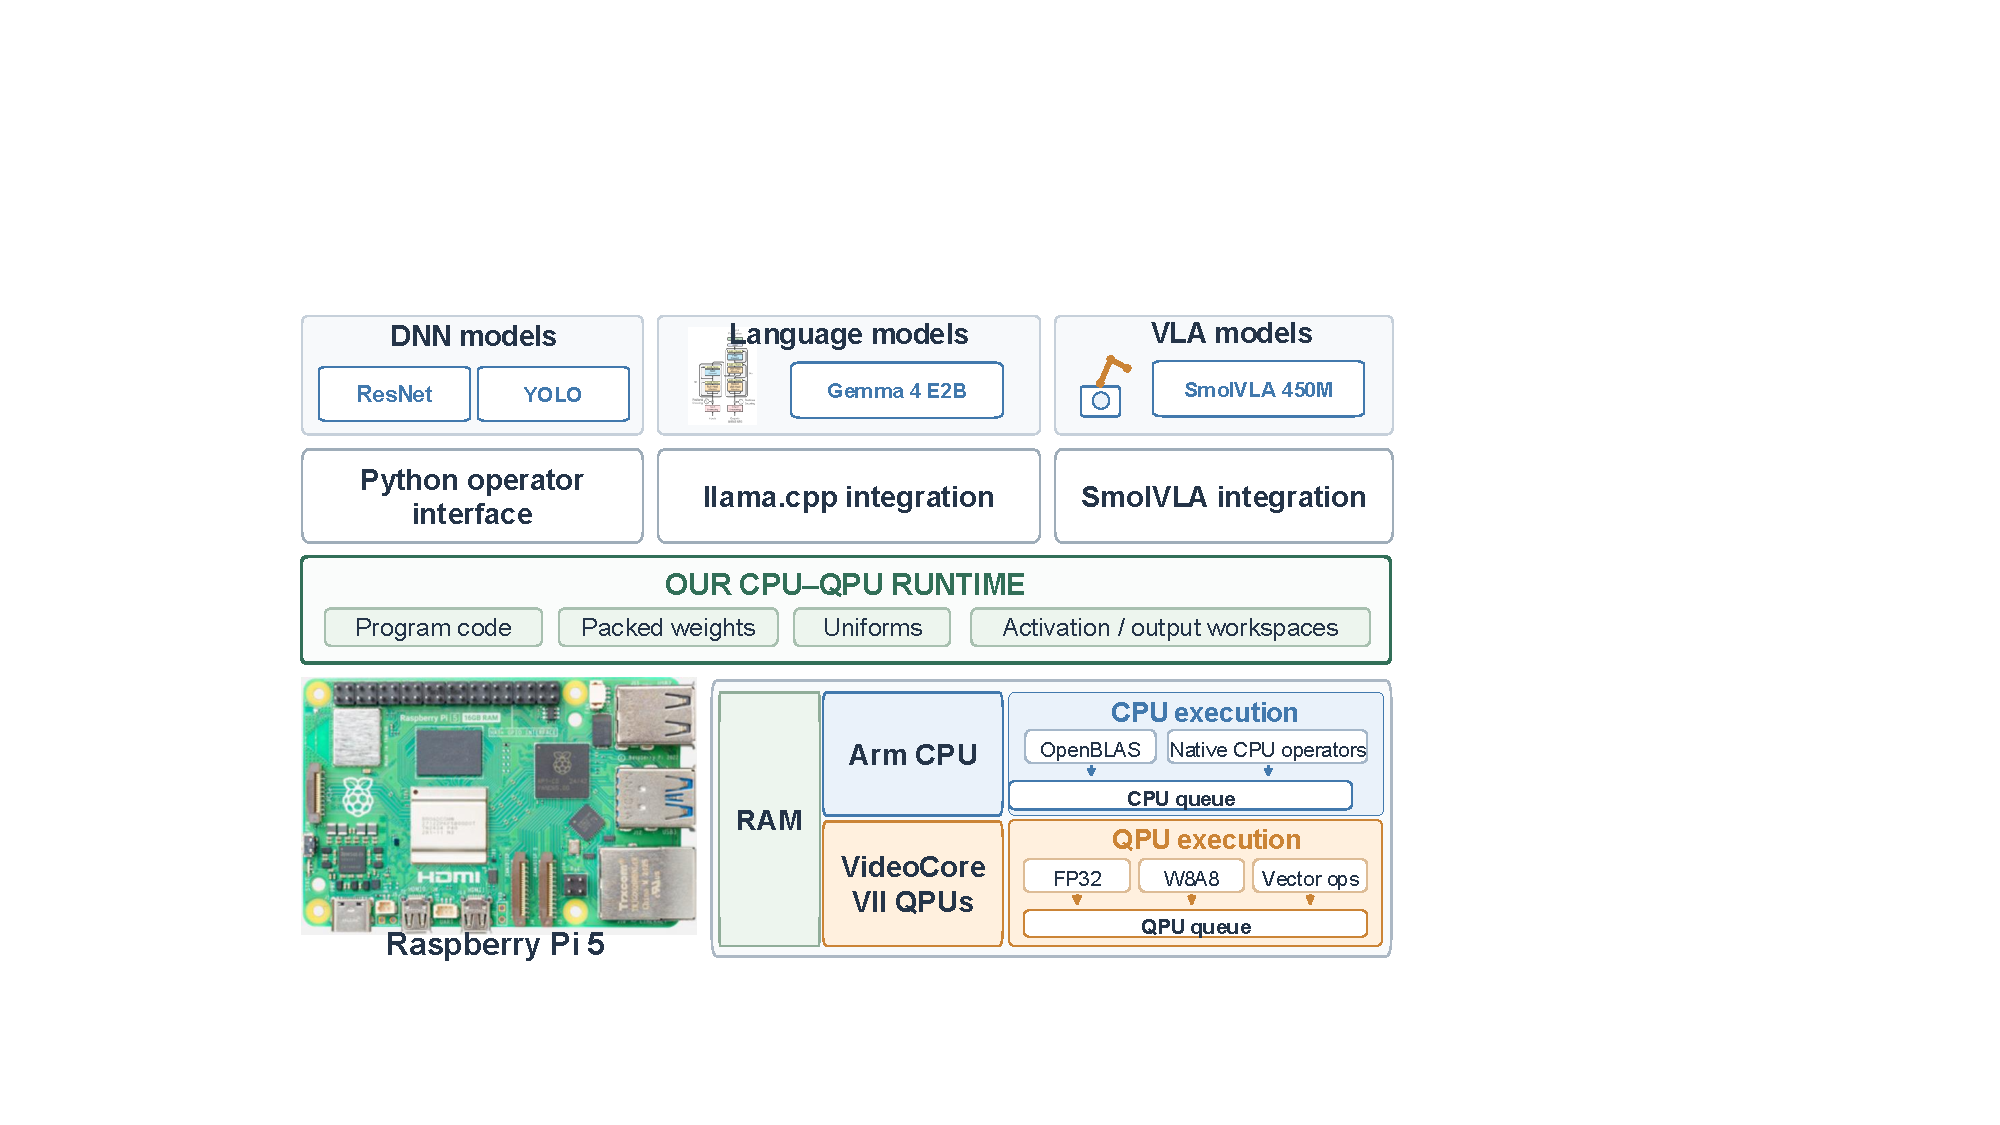
\includegraphics[width=0.95\linewidth]{figure1.pdf}
    \caption{Native CPU--QPU runtime on Raspberry Pi~5. Vision, language, and VLA workloads share persistent programs, weights, and workspaces, with separate CPU and QPU queues accessing shared physical memory.}
    \label{fig:overview}
\end{figure}


\section{Background and Related Work}
\label{sec:background}

Raspberry Pi~5 integrates four Arm Cortex-A76 CPU cores and a VideoCore~VII graphics processor within the BCM2712 system-on-chip~\cite{rpi5processor}. VideoCore~VII contains 12 programmable QPU cores that execute 16-lane vector instructions. Native programs access memory through the V3D interface and are launched through DRM V3D compute dispatches. The instruction set provides FP32 arithmetic, vector memory operations, and \texttt{v8dot}, which computes dot products over four signed bytes packed into each 32-bit word. The CPU and QPUs share physical memory, making it possible to place model weights, activations, and outputs in mapped allocations accessible to both processors.

Existing inference systems provide the technical context and the CPU baselines for our study. XNNPACK provides optimized operators for Arm CPUs~\cite{xnnpack}, while \texttt{llama.cpp} combines quantized model formats, architecture-specific CPU kernels, graph execution, and inference algorithms~\cite{llamacpp}. T-MAC demonstrates how matching low-bit representations to available CPU instructions can substantially improve LLM inference, including on Raspberry Pi~\cite{tmac}. ncnn provides mobile inference through optimized CPU kernels and Vulkan graphics execution~\cite{ncnn}, representing the conventional graphics route for embedded models. More broadly, Halide, TVM, Ansor, and Triton demonstrate how scheduling, tiling, data layout, and target-specific code generation determine application performance~\cite{halide,tvm,ansor,triton}. These systems motivate our whole-path evaluation, but do not provide native VideoCore~VII kernels or fine-grained CPU--QPU co-execution for Raspberry Pi~5 inference workloads.

At the lower level, \texttt{py-videocore7} supplies the assembler and V3D device interface used by our implementation~\cite{pyvideocore7}. VC4CL provides an OpenCL environment for the earlier VideoCore~IV architecture~\cite{vc4cl}, while V3DLib provides native VideoCore programming abstractions and kernel examples for documented VideoCore~IV and VI targets~\cite{v3dlib}. However, Raspberry Pi~5 presents a distinct implementation setting in which the CPU and QPUs share physical memory, while QPU execution relies on a target-specific instruction set and dispatch interface. Native QPU code must therefore coexist with representations and CPU implementations designed around different execution models: W8A8 maps directly to signed-byte dot products, GGML block formats~\cite{llamacpp} require format-specific unpacking and scaling, OpenBLAS targets dense numerical operations~\cite{openblas}, and CPU\_REPACK~\cite{llamacpp} couples packed representations with optimized Arm kernels.

Intra-layer FFN partitioning has established precedents: Megatron-LM splits intermediate channels and combines down-projection contributions~\cite{shoeybi2019megatron}; PowerInfer distributes hot and cold neuron execution between GPU and CPU~\cite{song2024powerinfer}; CoDL coordinates heterogeneous operator partitions and chains to reduce sharing costs~\cite{jia2022codl}. Our contribution is the native VideoCore~VII integration and its production CPU\_REPACK evaluation, building on the earlier QPU substrate~\cite{hadjiyianni2026qpu}, rather than introducing channel partitioning or operator-chain locality.

Recent Raspberry Pi inference studies investigate low-bit and ternary quantization for language models~\cite{llmpi}, INT8 deployment of convolutional detectors through TensorFlow Lite~\cite{boddu2025quantizedyolo}, and lightweight CPU implementations of spiking neural networks~\cite{derzhavin2025spiffy}. These approaches target model compression and application-specific execution without developing native CPU--QPU co-execution. Overall, to our knowledge, Raspberry Pi~5 currently lacks an AI-inference execution layer that combines native QPU kernels, persistent model state, packed representations, and concurrent execution within one model runtime.


\section{System Design and Implementation}

We examine how kernel design, data representation, and runtime scheduling jointly determine whether native QPU execution improves AI inference (Figure~\ref{fig:overview}). We build a CPU--QPU runtime to retain reusable state and coordinate concurrent work (Section~\ref{sec:arch}), generate kernels that exploit VideoCore~VII arithmetic and memory access (Section~\ref{sec:kernels}), and compose these operators across vision, language, and vision--language--action workloads (Sections~\ref{sec:dnn}-\ref{sec:vla}). 


\subsection{CPU–QPU Runtime Architecture}
\label{sec:arch}

We organize CPU--QPU execution around shared mapped tensors, persistent programs and workspaces, and calibrated placement with CPU recovery. Each candidate retains the workload's shape, layout, precision, and CPU implementation, with explicit ownership and dependencies coordinating preparation, execution, and synchronization.

\subsubsection{Mapped tensors, queues, and memory ownership}

We allocate V3D buffer objects and map them into the host process so CPU and QPU code can access the same storage. In each tensor, we record its dtype, shape, strides, byte offset, and allocation ownership; CPU code uses a NumPy-compatible host view, while QPU programs receive the corresponding device address. Slicing adjusts the view's offset and byte range without allocating or copying data. We tie view validity to the underlying allocation: closing it invalidates all derived views, even if the storage is later reused. 

For each operation, we declare the byte ranges it reads and writes, making ownership explicit and enabling checks for conflicting or invalid accesses. We use separate in-order queues for CPU and QPU tasks and connect them through events that record submission, completion, and failure. We declare dependencies so QPU tasks wait for CPU preparation, overlap independent CPU work, and signal when their outputs are ready for dependent operations. We handle V3D dispatch and synchronization in a queue worker, providing the application with an asynchronous task interface.

\subsubsection{Persistent plans and shared-memory execution}

We retain assembled QPU programs, uniforms (kernel parameters), transformed weights, address tables, padding metadata, and scratch buffers in persistent plans because inference repeatedly applies the same programs and weights to changing activations. We perform activation-independent setup once during plan construction. At each invocation, we prepare the current input, update the required uniforms, submit CPU and QPU tasks, and synchronize when their outputs are needed. For tensors already in mapped storage, both processors access the same allocation without a separate host-to-device copy. For framework-owned tensors, we support staging into the persistent QPU workspace. 

For language-model operations on GGML tensors, we use cacheable DMA-buffer mappings and explicit CPU-access synchronization, with AArch64 NEON routines that deinterleave repacked activations into the QPU input format. We account for these conversion and synchronization operations in invocation time. We also preserve tensor alignment throughout persistent allocation. The affected vector kernels use the Texture Memory Unit (TMU) for memory access and require 256-byte-aligned tensor bases. Because our allocator assigns storage linearly, a small uniform allocation can misalign subsequent tensors. We therefore reserve 256-byte uniform blocks for these vector stages and tiled FP32 kernels, preserving alignment for later activation and workspace allocations. We record both logical tensor dimensions and physical padded layouts in each plan.


\subsubsection{CPU--QPU partitioning and placement}

We partition work along dimensions that preserve independent output ownership: rows for multi-row projections or output columns for single-row projections. Both processors share read-only inputs and write disjoint output regions, requiring synchronization without an arithmetic merge. We register supported partition axes and alignment constraints for each operator. Partition axes follow the operator semantics. For grouped convolution, for example, we must ensure group-aligned output ranges, while a depthwise operator cannot use an arbitrary output-channel split.

We separate an implementation's supported configurations from its eligibility for automatic placement. Calibration records identify the exact operation, dimensions, dtype, layout, arithmetic mode, partition, implementation revision, numerical validation, and measured latency. We select among eligible CPU-only, QPU-only, and hybrid configurations: an unseen shape, unmatched layout, or changed implementation uses the CPU path until new evidence is available. This exact-match policy captures performance changes caused by vector alignment, tail handling, and shifts in the CPU/QPU critical path. Recovery follows the same ownership contract. If a QPU task fails after receiving ownership of an output region, we recompute that region on the CPU before signaling completion, ensuring that dependent operations receive a complete output. Downstream operations therefore observe a complete logical output regardless of the point at which QPU execution fails.


\subsection{Native Kernel Generation}
\label{sec:kernels}

We generate native VideoCore~VII programs by matching each supported operator's dtype, logical and physical dimensions, layout, and partition range to a validated kernel family. We instantiate the tile and workgroup geometry, emit instructions through the Python assembly interface, and retain the program, uniforms, and workspace requirements in a persistent plan. We design these schedules around the QPU's 16-lane execution width, register capacity, TMU access patterns, and arithmetic instructions, using FP32 operations or packed signed-byte dot products for W8A8. This approach connects instruction-level choices to the tensor layouts and CPU--QPU partitions used by the runtime across matrix operations, vector and reduction stages, spatial preprocessing, pooling, convolution lowering, attention components, and neural-network epilogues.

\subsubsection{FP32 and integer kernels}

We generate FP32 GEMM kernels around a logical $16\times16\times4$ tile: sixteen output rows, sixteen output columns, and four reduction values per iteration. We keep sixteen accumulator vectors in registers, pipeline TMU requests, reuse loaded operands, rotate values across lanes, and interleave address arithmetic with FP32 multiplication and addition. We prepare transformed, transposed, and padded weights once in the persistent plan. For aligned projections, we read mapped activations and write mapped outputs directly; otherwise, we use padded dimensions and explicit staging. Kernel selection therefore accounts for logical and physical dimensions, tensor-base alignment, and partition range. 

For INT32 GEMM, we use \texttt{smul24}, restrict operands to the signed 24-bit range, and check that accumulation fits in INT32, including intermediate values in compound operators. We execute INT16 convolution by widening inputs and weights to this validated integer representation before dispatch. For bandwidth-oriented kernels, we use four contiguous 32-bit words per SIMD lane and distribute complete vector stripes across the available QPUs. We reuse this access pattern for copy, elementwise minimum and maximum, residual addition, activation, and pooling, with operator-specific arithmetic and stores. For prepared pooling, we additionally cache source-address metadata and select the largest QPU count, up to twelve, that exactly divides the vector stream.


\begin{figure}[t!]
    \centering
    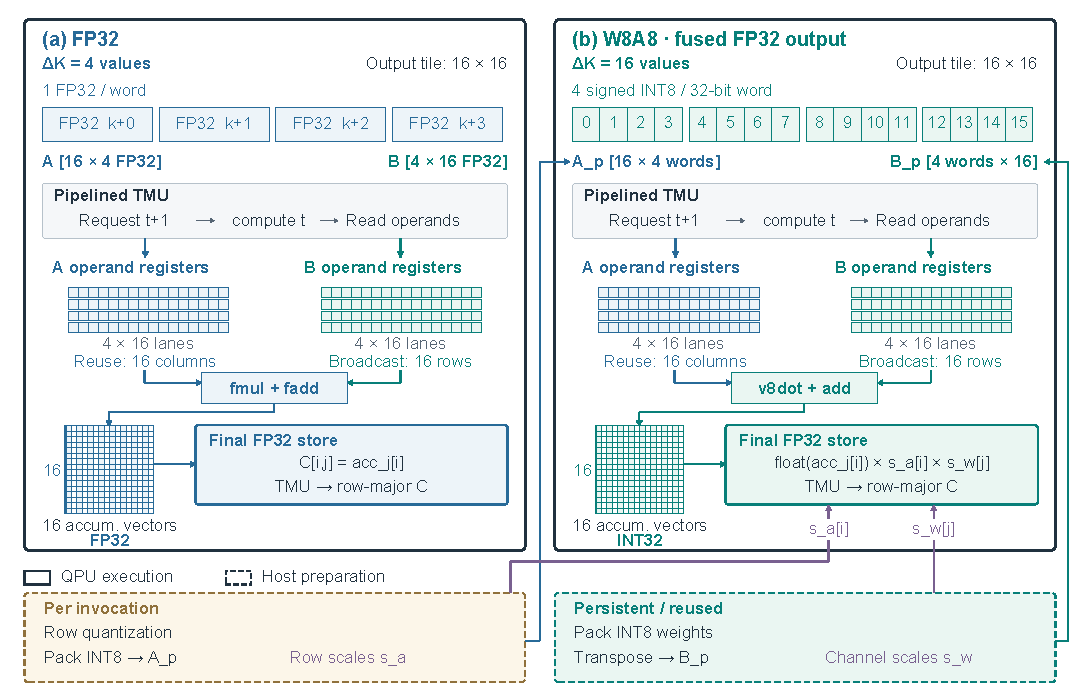
\includegraphics[width=0.95\linewidth]{figure2.pdf}
    \caption{FP32 and W8A8 matrix-kernel dataflows. FP32 uses a $16\times16\times4$ tile; W8A8 uses a $16\times16\times16$ tile with packed byte-dot arithmetic, persistent weights, and fused output scaling.}
    \label{fig:placeholder}
\end{figure}


\subsubsection{Instruction-matched W8A8}
\label{sec:w8-design}

We use symmetric W8A8 quantization~\cite{jacob2017quantization} with one dynamic scale per activation row and one persistent scale per output channel. Following established quantization granularities~\cite{smoothquant}, we round scaled values to the nearest integer with ties to even, clip to $[-127,127]$, and accumulate products in INT32. We compute each scale from the row or channel's maximum absolute value divided by 127, with a minimum scale of $1/127$. This avoids division by zero and sets a minimum quantization step for small-magnitude inputs. We reject configurations whose padded reduction length could overflow INT32 under the conservative bound $K_{\mathrm{pad}}127^2 \leq 2^{31}-1$. Because the row and channel scales remain constant throughout each reduction, we apply them after integer accumulation.

We pack four signed INT8 values into each 32-bit word to match VideoCore~VII's \texttt{v8dot} instruction~\cite{pyvideocore7} and generate a $16\times16\times16$ tiled kernel with pipelined activation and weight loads. We retain packed weights and per-channel scales across invocations and quantize each activation directly into the mapped input buffer consumed by the QPU, avoiding an additional copy of the quantized tensor. We fuse row- and channel-scale application into the FP32 output store to eliminate a separate traversal of the INT32 accumulator matrix. We retain CPU and standalone QPU scale-application paths so we can measure the effect of this fusion separately from the integer kernel and activation preparation.


\subsection{Vision and Convolutional Model Execution}
\label{sec:dnn}

To implement native CPU--QPU execution for convolution-related layouts, we follow mature inference libraries such as cuDNN as guidance for organizing vision computation into reusable operators and mapping convolution to efficient matrix kernels~\cite{chetlur2014cudnn}. Specifically, we follow cuDNN design principles to build native QPU operators for convolution, pooling, residual and elementwise operations, activation, normalization, resize, gather, patch extraction, and dense projection, supporting classification, detection, and image preprocessing. 

We implement convolution over NCHW activations and OIHW weights using the established convolution-to-GEMM lowering approach~\cite{chetlur2014cudnn}, allowing spatial operators to reuse our FP32 and W8A8 matrix kernels. We specialize $1\times1$ pointwise and depthwise execution to reflect their distinct computational structures~\cite{howard2017mobilenets}: we pack spatial locations directly into matrix rows without expanding spatial windows, and we reduce packed spatial windows independently by channel, respectively. We retain packed weights, padding metadata, and reusable workspaces in prepared convolution plans to amortize activation-independent preparation across inputs. We compose these reusable primitives into compact classification pipelines and exercise production-shaped operators from larger vision models, following standard operator-library frameworks~\cite{chetlur2014cudnn}. 


\subsection{Language-Model Execution}
\label{sec:llm}

To implement native CPU--QPU execution for language models, we integrate and extend the established \texttt{llama.cpp} runtime. Its optimized Arm kernels provide a competitive CPU baseline to evaluate against~\cite{llamacpp}. 


\subsubsection{Packed and converted representations} 

For GGML Q4\_0, Q4\_K, Q6\_K, and Q8\_0 weights, we preserve the original block scales and quantization semantics while retaining decoded metadata and rearranged integer fields for reuse~\cite{llamacpp}. We incorporate format-specific unpacking, scaling, and activation handling into the native kernels without expanding the complete weight matrix to FP32. 

We also implement persistent column-W8 conversion with per-output-column weight scales and dynamic per-row activation quantization. This simplifies QPU arithmetic at the cost of additional resident storage and an additional quantization approximation. For dense CPU execution, we convert supported weights to FP32 and invoke OpenBLAS~\cite{openblas}. Alongside the optimized CPU\_REPACK path~\cite{llamacpp}, these alternatives let us examine representation and execution placement within the same model graph. We apply numerical and model-output checks separately to each representation.

\subsubsection{Graph execution and projection overlap}

We implement four execution scopes to examine how graph boundaries affect CPU--QPU execution. For \emph{direct node execution}, we register native matrix or attention kernels as QPU implementations of supported graph nodes. For \emph{inline activation execution}, we invoke QPU GEGLU from the CPU graph executor while preserving the original graph placement, avoiding the scheduler transitions introduced by assigning individual operations to a separate device backend. The native C runtime manages persistent programs, weights, uniforms, staging buffers, synchronization, and recovery for these paths.

For \emph{asynchronous projection overlap}, we assign disjoint output-column ranges to the CPU and QPU, dispatch the QPU slice before independent CPU work, and synchronize before the combined projection is consumed. We support native GGML and converted column-W8 weights under the same overlap mechanism to examine how representation affects concurrent execution. We record executed layers, shapes, programs, partitions, dispatches, and fallbacks to verify the path exercised by each request. 



\subsubsection{Channel-partitioned FFN execution}
\label{sec:ffn}

Our node-level experiments showed that accelerating an individual projection or activation could leave preparation, synchronization, and the following operation on the critical path. We therefore extend CPU--QPU partitioning across gate projection, up projection, GEGLU, and down projection. The key observation is that intermediate FFN channels can be computed independently through the activation, after which the down projection sums their contributions. We assign each processor a channel slice through the complete sequence, retaining intermediate values locally and combining only the final partial outputs. 

To this end, we divide the intermediate channels into disjoint CPU-owned indices $J_c$ and QPU-owned indices $J_q$. If $H$ denotes the GEGLU activation and $W_d$ the down-projection weights, the decomposition is
\begin{equation}
Y =
H_{[:,J_c]}W_{d[J_c,:]}
+
H_{[:,J_q]}W_{d[J_q,:]}.
\end{equation}
Each processor computes its gate and up projections, activation, and down-projection contribution for its assigned channels. The corrected confirmation fixes the QPU share at one eighth before evaluation; later exploratory screening does not establish an optimum. The execution boundary follows from this channel independence and the additive structure of the down projection.

We implement this within CPU\_REPACK~\cite{llamacpp} to reuse the activation representation already prepared by the CPU runtime. We pass the CPU partition width and physical source-row stride separately to the activation quantizer, allowing CPU\_REPACK to process its channel slice directly without an additional compacting copy. We retain the QPU's GEGLU-to-Q8 intermediate for its down projection, avoiding a return to host storage between these stages. The CPU and QPU produce hidden-size partial outputs that we add at the final join. This design addresses both representation preparation and intermediate synchronization while preserving the optimized CPU path for its channel slice. We validate the combined output against CPU execution, accounting for intermediate quantization and the changed accumulation order.


\subsection{Vision--Language--Action Model Execution}
\label{sec:vla}

VLA models are an important edge-AI workload for robotics, motivating us to investigate their CPU--QPU execution opportunities on Raspberry Pi~5. To this end, we extend our runtime to support VLAs based on SmolVLA~\cite{smolvla}. 

\subsubsection{Policy execution and placement} 

We incorporate the compact, 450M-parameter SmolVLA policy, by integrating its visual encoding and flow-matching action-generation architecture~\cite{smolvla} and mapping its computation onto our native CPU--QPU operators. We resize and normalize three RGB observations, encode them with SigLIP~\cite{siglip}, and apply pixel shuffle and projection to obtain visual features. We then populate the KV cache and run ten Euler steps through the action expert to produce a $50\times6$ action sequence. We reuse weights and cached state across these steps while preparing the changing activations.

We provide QPU paths for image preprocessing, projections, normalization, activations, residual operations, embedding, RoPE, attention stages, and pixel shuffle. We partition rows, output columns, or query heads according to operator dependencies, while the CPU handles mask construction, time embedding, Euler updates, and final slicing. We preserve the upstream SmolVLA preprocessing and numerical semantics and validate parameter shapes and dtypes during model loading~\cite{smolvla}. Common deterministic replays and output checks let us compare FP32 and dynamic W8A8 representations under CPU, QPU, hybrid, and calibrated placement.


\begin{figure}[t]
    \centering
    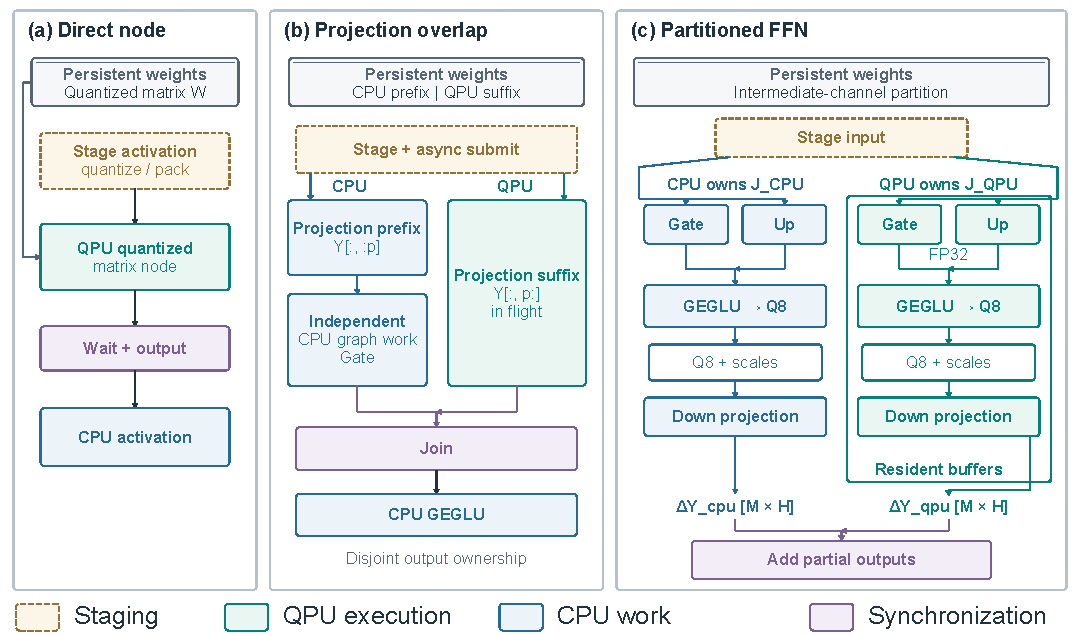
\includegraphics[width=0.9\linewidth]{figure3.pdf}
    \caption{Language-model execution scopes: (A) direct QPU node execution, (B) asynchronous projection overlap, and (C) channel-partitioned FFN execution with resident intermediates and addition of hidden-size partial outputs.}
    \label{fig:integration}
\end{figure}


\section{Evaluation Methodology}
\label{sec:method}

We investigate three connected questions: which layouts and numerical representations make complete QPU operators competitive; how preparation, persistence, synchronization, and partitioning affect concurrent CPU--QPU execution; and how much of an operator-level improvement reaches a complete AI workload. We examine these questions progressively, from prepared kernels and complete operators to concurrent execution, model regions, and complete requests.

\subsection{Execution Boundaries and Timing}

To quantify the latency effect of CPU--QPU concurrency, we must include all work required to produce a usable output. We therefore follow established accelerator benchmarking practices for asynchronous execution~\cite{pytorchbenchmark}. We distinguish prepared kernel execution from complete operator latency, which includes dynamic input preparation, submission, execution, synchronization, and output handling. 

Concurrent measurements include both processors' completion and the final join; model-region and request measurements additionally include the enclosing computation and runtime boundaries. Steady-state measurements reuse programs, weights, and workspaces, while cold-start measurements include their construction~\cite{marculescu2018hardwareaware}. For disjoint output partitions, we interpret hybrid latency as
\begin{equation}
T_{\mathrm{hybrid}}
\approx
T_{\mathrm{prep}}
+
\max\!\left(T_{\mathrm{CPU}},T_{\mathrm{QPU}}\right)
+
T_{\mathrm{join}}.
\end{equation}
Here, preparation precedes concurrent execution, and the join completes any remaining synchronization and result handling. We measure CPU and QPU durations during co-execution because shared-memory contention can change their performance relative to isolated runs. We select partitions by complete latency through the join; equal row counts or operation counts need not balance execution time.

Operator experiments perform warm-up iterations before collecting repeated steady-state samples and report median latency. For channel-partitioned FFN execution, we fix the QPU channel fraction at one eighth before confirmation and use four CPU threads. Full-prompt measurements use five independent processes per implementation at each of $M=129$ and $M=257$, with one timed prompt per process after warm-up. The cached-request experiment uses 15 independent process pairs. Each server first populates a 512-token prefix, then processes a 128-token tool-result suffix and returns one greedy token. Prefix population precedes timing; the request includes five replayed prefix tokens and has physical FFN $M=129$. We randomize process order, disable swap, and check temperature, throttling, and competing workloads at the measurement boundaries. We compute 95\% confidence intervals using 10,000 bootstrap resamples, independently resampling the full-prompt process groups and preserving pairs for cached requests.



\subsection{Experimental Setup and Campaign}

\subsubsection{Experimental Platform}
We run experiments on an actively cooled 8\,GB Raspberry Pi~5 with four Cortex-A76 CPU cores ($\approx$2.4\,GHz) and 12 VideoCore~VII QPUs. The FP32 campaign uses NumPy~2.2.2 with \texttt{scipy-openblas}~0.3.28 and PyTorch~2.11.0, with four OpenBLAS, OpenMP, and PyTorch intra-operation threads. The separate dense-BLAS campaign uses OpenBLAS~0.3.29. We record the V3D clock, temperature, throttling indicators, process state, memory pressure, and swap activity.

% Earlier operator measurements use the \texttt{ondemand} governor; we retain this distinction in the reported configurations.

\subsubsection{Baselines}
We compare FP32 operators against the faster measured NumPy or PyTorch implementation for each exact shape. NumPy matrix multiplication uses OpenBLAS, while native PyTorch convolution provides the CPU reference for spatial operators. Quantized language-model nodes use \texttt{llama.cpp}'s optimized CPU\_REPACK implementation with production repacking enabled. CPU thread counts follow the relevant execution configuration, including one-thread production nodes where applicable. An OpenBLAS-enabled build evaluates dense matrix execution with converted FP32 weights, including the conversion and graph-transition costs incurred within the measured boundary.

We evaluate QPU-only execution and supported aligned CPU--QPU partitions. The model-runtime experiments additionally compare direct node execution, inline QPU invocation, asynchronous projection overlap, and channel-partitioned FFN execution. We identify the CPU implementation used by each hybrid slice: the generic matrix runtime uses NumPy, while native language-model paths use their recorded GGML implementation. This distinction matters when the fastest full-operator CPU reference differs from the implementation used inside a partition.

\subsubsection{AI workloads}

We evaluate three workload families. For vision, we use compact classification pipelines and production-shaped convolution operators from YOLO~\cite{redmon2016yolo}, covering pointwise, $3\times3$, and depthwise execution. Transformer operator experiments cover projections, normalization, activations, RoPE, and attention across single-token decode and multi-token prefill. For production language-model execution, we use Gemma~4 E2B~\cite{gemma4} in \texttt{llama.cpp}, with a Q4\_K\_XL model whose evaluated FFN weights use Q4\_0 tensors. The attention sweep uses context lengths of 512 and 4096 with query-row counts $M\in\{65,257\}$. For VLA execution, we use the 450M-parameter SmolVLA policy~\cite{smolvla}.

To assess whether native execution preserves application-level outputs, we evaluate matched CPU and CPU--QPU runs on downstream benchmarks: We subsample 1k MMLU questions for Gemma and 5k $128\times128$ ImageNet images for ResNet-18, selecting five images per class by deterministic hashing. For SmolVLA, we compare complete $50\times6$ action sequences against upstream FP32 outputs on 100 observations drawn from ten episodes, retaining identical observations, state, language inputs, masks, and initial flow noise. For object detection, we subsample 1k COCO val2017 images for YOLOv8n, using matched $640\times640$ inputs and identical confidence filtering, non-maximum suppression, and detection limits for CPU and QPU execution. We report bounding-box AP, AP$_{50}$, recall, and detection agreement.



\subsection{Numerical and Model Validation}

To validate correctness at the same execution boundary used for performance measurement, we implement explicit programmatic checks against reference outputs, following established numerical-validation practices for exact integer arithmetic and tolerance-based floating-point comparisons~\cite{pytorchtesting,pytorchnumerics}. INT kernels are checked against their specified accumulation contract, and FP32 kernels against independent NumPy or PyTorch references using operation-specific tolerances. Partition tests check the computed output and verify that QPU execution preserves CPU-owned regions. For channel-partitioned FFNs, we check the combined output after adding both processors' contributions. 

We validate quantized execution against a CPU implementation of the same quantization contract and measure deviation from the FP32 or native model reference. We check generated tokens or action outputs for the evaluated inputs, report failures against the tolerance used during each experiment, and retain separate validation results for native-format and converted representations. We report paired accuracy differences with bootstrap confidence intervals for MMLU and class-stratified paired intervals for ResNet-18, together with numerical action agreement for SmolVLA.

\subsection{Calibration and Reproducibility}

To prevent tuning bias and make results reproducible, we separate partition calibration from held-out evaluation and record each configuration's operation, shape, layout, representation, partition, implementation revision, numerical result, and complete-operation latency. We match weights, inputs, cache state, and deterministic generation settings between CPU and candidate runs, preserving quantization settings for same-representation comparisons and documenting conversion for W8 and dense-FP32 alternatives.

To verify that each request executes the intended path, we record dispatch counts, program identity, selected partitions, and fallback events. We retain environment records and available component timings to explain performance differences. The anonymized implementation supports generating these records, raw timing samples, and execution traces to facilitate reproduction and verification under the documented configurations.



\section{Results}
\label{sec:results}

We evaluate native CPU--QPU execution across matrix, vector, reduction, convolution, and attention operators, then examine how these results carry into language-model execution and VLA memory requirements. Unless otherwise stated, speedup is CPU latency divided by candidate latency.

\subsection{Native Operator Performance}

\subsubsection{FP32 execution: layout, partitioning, and fusion}

To identify where native execution complements optimized CPU kernels, we compare complete FP32 operators across projection shapes and vector workloads. The projection campaign identifies ten configurations with speedups of 1.117--1.356$\times$. Four $M=16$ cases select QPU-only execution, while all six selected $M=64$ cases use a sixteen-row QPU prefix with a NumPy CPU tail. Table~\ref{tab:fp32-main} reports representative configurations. These measurements use the \texttt{ondemand} governor and characterize the recorded operator campaign.

\begin{table}[t]
\centering
\caption{Complete-operator FP32 projection latency under the \texttt{ondemand} governor. Shapes are $M\times K\times N$; ``16 rows'' assigns a 16-row prefix to QPU, the remainder to CPU.}
\label{tab:fp32-main}
\small
\begin{tabular}{@{}lrrr@{}}
\toprule
Shape; placement & CPU ms & Candidate ms & Speedup \\
\midrule
$16\times1536\times512$; QPU & 1.750 & 1.472 & 1.189$\times$ \\
$16\times512\times32000$; QPU & 32.774 & 24.166 & 1.356$\times$ \\
$64\times2816\times1024$; 16 rows & 7.052 & 6.165 & 1.144$\times$ \\
$64\times1024\times2816$; 16 rows & 7.398 & 6.083 & 1.216$\times$ \\
$64\times1024\times1024$; 16 rows & 3.344 & 2.484 & 1.346$\times$ \\
\bottomrule
\end{tabular}
\end{table}

Vector operations reveal a sharper dependence on layout. At 4,194,048 elements, minimum and maximum achieve 1.550$\times$ and 1.517$\times$ speedups over NumPy. At the nearby length 4,194,240, they achieve only 0.908$\times$ and 0.909$\times$. Inspection of the selected kernels shows that the larger length fails the current exact-stripe predicate and selects scalar execution (Figure~\ref{fig:stripes}). The discontinuity therefore comes from kernel selection: a small change in element count changes how the operation is distributed across lanes and QPUs.

\begin{figure}[t]
    \centering
    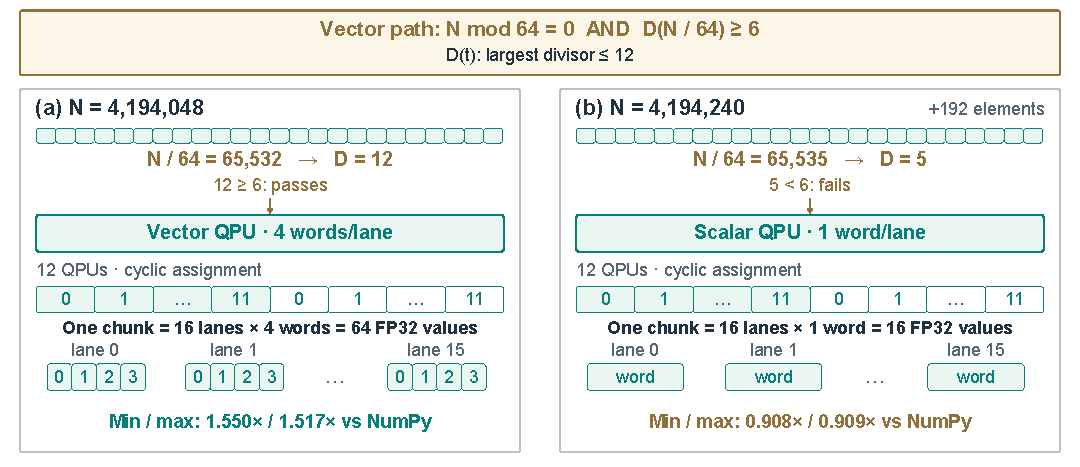
\includegraphics[width=\linewidth]{figure4.pdf}
    \caption{Exact-stripe kernel selection. Length 4,194,048 permits twelve-way vector execution; the neighboring length 4,194,240 fails the vector-selection predicate and uses the scalar path.}
    \label{fig:stripes}
\end{figure}

Prepared pooling benefits from selecting the largest QPU count, up to twelve, that exactly divides the vector stream. At input shape $1\times48\times128\times128$, average and maximum pooling achieve 1.645$\times$ and 1.640$\times$ speedups. Fusion provides another opportunity: bias-plus-ReLU on $16\times262128$ values achieves 1.920$\times$ against the recorded NumPy implementation by combining its two array passes into one QPU traversal. Together, these experiments show how exact work distribution and reduced memory traversal contribute alongside arithmetic throughput.

\subsubsection{Quantized execution and operator composition}

We next examine whether matching arithmetic to \texttt{v8dot} expands the useful projection range. The earlier W8A8 campaign reports selected improvements of 1.21--1.68$\times$ at $M=64$ with hidden size 1024, and 1.09--1.30$\times$ at $M=128$ with hidden size 2048. These comparisons include the change from FP32 CPU execution to W8A8 QPU execution. They are retained measurements of the corresponding implementations; records whose source hashes no longer match are excluded from current automatic placement.

To assess composition, we compare the mixed one-layer runtime with its FP32 NumPy reference. Three tuning configurations achieve 2.86$\times$, 1.54$\times$, and 1.16$\times$, while a held-out configuration with 256 tokens and hidden size 2048 achieves 0.83$\times$. Evaluated decode compositions achieve only 0.38--0.60$\times$. Thus, the arithmetic improvement depends on the surrounding stages and available row parallelism, even within the same model family.

A producer-consumer experiment isolates this effect more directly. We compare a resident GEGLU-to-Q8 producer with the sequence that includes its Q4 down projection (Table~\ref{tab:producer-consumer}). At $M=257$, the producer improves from 6.343\,ms on CPU to 5.568\,ms on QPU, a 1.139$\times$ speedup. Adding the down projection changes the comparison to 18.904\,ms versus 70.637\,ms, or 0.268$\times$. The resident intermediate removes a host exchange, but the consumer dominates the resulting sequence.

\begin{table}[t]
\centering
\caption{Prepared GEGLU-to-Q8 producer and producer-plus-Q4-down-projection latency. Speedup compares CPU and QPU execution of the combined sequence.}
\label{tab:producer-consumer}
\small
% \resizebox{\columnwidth}{!}{%
\begin{tabular}{@{}rrrrrr@{}}
\toprule
& \multicolumn{2}{c}{Producer} &
\multicolumn{2}{c}{Producer + down} & \\
$M$ & CPU ms & QPU ms & CPU ms & QPU ms & Speedup \\
\midrule
65  & 1.564 & 1.697 & 4.555 & 21.104 & 0.216$\times$ \\
129 & 3.157 & 3.005 & 9.542 & 37.582 & 0.254$\times$ \\
257 & 6.343 & 5.568 & 18.904 & 70.637 & 0.268$\times$ \\
\bottomrule
\end{tabular}
% }
\end{table}

Native GGML execution adds format-specific unpacking, block scales, and activation-layout processing around the integer dot product. The small-row experiments remain CPU-favorable, including a production MTP node with $K=256$ and $N=2048$: its QPU path takes approximately 350\,$\mu$s versus 25\,$\mu$s for the relevant one-thread CPU\_REPACK implementation. Removing graph-scheduler transitions leaves this operator deficit intact. These results direct subsequent optimization toward larger execution regions with reusable representations.

\subsubsection{Convolution and attention}

We evaluate convolution and attention to test whether the matrix-kernel improvements extend to operators with spatial preparation or coupled reductions. Against native PyTorch FP32 convolution, the earlier GEMM-backed YOLO cases achieve approximately 0.13$\times$ for pointwise convolution, 0.064$\times$ for $3\times3$, and 0.012$\times$ for depthwise convolution. Pointwise execution avoids spatial-window duplication but still incurs layout preparation; general convolution adds \texttt{im2col} expansion, while depthwise convolution offers limited reuse within a dense reduction tile, motivating specialized spatial dataflows. %The later W8A8 depthwise path changes the reduction structure but still materializes and packs spatial windows, so its preparation costs must also be included when evaluated. 

To assess whether batching amortizes attention dispatch costs, we combine query rows and heads into one QPU launch for Gemma~4 E2B~\cite{gemma4}, using online softmax. With 11 samples per case and a three-thread CPU reference, the QPU achieves 0.588$\times$ and 0.328$\times$ at context 512 for $M=65$ and $M=257$, respectively. At context 4096, the corresponding ratios are 0.565$\times$ and 0.335$\times$. Consolidating dispatches therefore leaves substantial kernel execution costs.

The Q4 experiment quantifies launch consolidation for two projection phases. Combining them into one dispatch reduces the narrow-suffix latency from 48.176\,ms to 46.502\,ms and the wide-suffix latency from 96.187\,ms to 92.776\,ms, approximately 1.036$\times$ relative to two QPU dispatches. Across these experiments, reducing launch count helps, but competitive convolution and attention also require changes to preparation, memory access, and reduction schedules.

\subsection{Performance within Model Runtimes}

\subsubsection{CPU representation and baseline selection}

To establish the relevant CPU comparison, we evaluate the native CPU\_REPACK path alongside an OpenBLAS-enabled \texttt{llama.cpp} build using the same model, software revision, and four CPU threads. In the recorded three-sample prompt-processing comparison, CPU\_REPACK is 15.77$\times$ faster at 33 prompt tokens and approximately 3.03$\times$ faster at 513--1025 tokens. The dense BLAS configuration converts supported quantized weights to FP32 and introduces CPU/BLAS graph transitions. These measurements capture the complete path, including matrix multiplication costs.

Partitioning the OpenBLAS FFN across CPU and QPU yields latency ratios of 1.18--1.38$\times$ relative to that dense CPU path. The comparison also changes activation precision: the OpenBLAS path uses dequantized Q4 weights with FP32 activations, while the QPU path uses Q8 activations. The recorded mean absolute differences of 0.10--0.14 and maximum differences of 1.85--5.95 must therefore be assessed as part of this representation change. They do not isolate an implementation error, and application-level checks are needed to establish acceptable output quality.


\subsubsection{Projection overlap and request latency}
\label{sec:overlap-results}

To determine whether concurrent execution shortens the request, we inspect the overlap between QPU projection work and independent CPU computation. The native \texttt{ffn\_up} path verifies execution across all 35 relevant layers. At $M=257$ with one-quarter of the output assigned to the QPU, its complete work takes 40.66\,ms per layer, while overlapping CPU work occupies 21.43\,ms. The resulting 19.23\,ms QPU tail contributes approximately 0.673\,s across the 35 layers (Figure~\ref{fig:overlap}).

\begin{figure}[t]
    \centering
    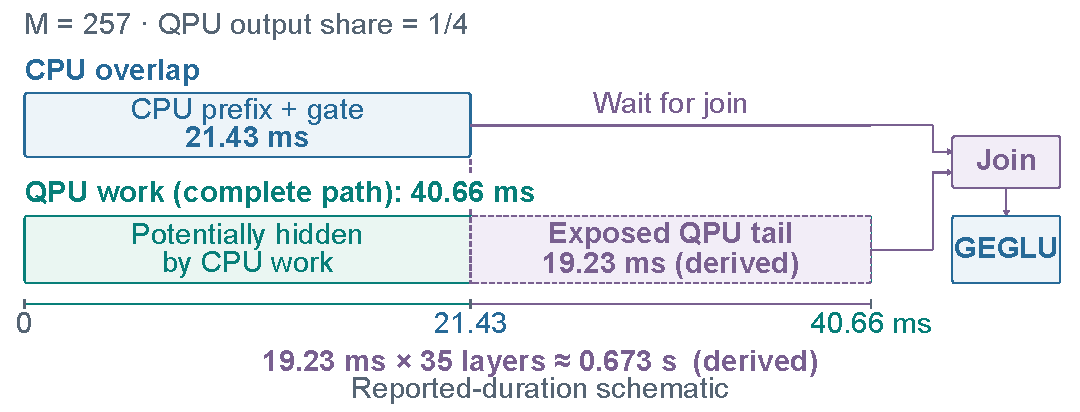
\includegraphics[width=\linewidth]{figure5.pdf}
    \caption{Measured projection overlap at $M=257$ with one quarter of the output assigned to the QPU. Its 40.66\,ms execution overlaps 21.43\,ms of CPU work, leaving a 19.23\,ms tail before the join.}
    \label{fig:overlap}
\end{figure}

The partition controls both CPU work removed and QPU work exposed. A smaller QPU share shortens the tail but leaves more computation on the CPU; a larger share can make QPU completion dominate the request. We therefore evaluate the selected partitions through complete requests, including preparation and synchronization.

Table~\ref{tab:requests} reports the converted column-W8 projection path. The $M=129$ and $M=257$ configurations each use five held-out CPU/candidate session pairs following separate calibration. At $M=257$, the measured speedup is 1.0161$\times$, but its bootstrap interval includes parity. The $M=513$ screening result is 1.0143$\times$ from one held-out pair. These measurements show limited request-level benefit from projection overlap under the evaluated configurations.

\begin{table}[t]
\centering
\caption{Complete-request latency for column-W8 \texttt{ffn\_up} overlap. $M$ is the observed projection row count. Confidence intervals use paired session resampling; the single-pair screen has no interval.}
\label{tab:requests}
\small
\resizebox{\columnwidth}{!}{
\begin{tabular}{@{}rrrrll@{}}
\toprule
$M$ & CPU ms & Candidate ms & Speedup & Bootstrap 95\% interval & Sessions \\
\midrule
129 & 3019.758 & 3021.002 & 0.9996$\times$ & [0.9466, 1.0236] & Five pairs \\
257 & 5603.841 & 5515.050 & 1.0161$\times$ & [0.6587, 1.1098] & Five pairs \\
513 & 9053.511 & 8925.507 & 1.0143$\times$ & Not estimated & One pair \\
\bottomrule
\end{tabular}
}
\end{table}

The evaluated requests produce identical greedy token IDs and verify the expected QPU dispatches without CPU fallback. The multi-session intervals include 1.0, and neither configuration meets the 1.05$\times$ request-level promotion threshold. Together with the overlap trace, these results motivate moving more producer--consumer work inside each processor's assigned region.

\begin{table}[t]
\centering
\caption{Channel-partitioned FFN latency against CPU\_REPACK. Prompts use five processes per implementation; cached requests use 15 process pairs. Each cached request adds 128 tokens to a prepopulated 512-token prefix and returns one token; prefix population is excluded.}
\label{tab:ffn-requests}
\small
\resizebox{\columnwidth}{!}{%
\begin{tabular}{@{}lrrrrl@{}}
\toprule
Workload & CPU (ms) & CPU--QPU (ms) & Latency reduction & Speedup & Bootstrap 95\% CI \\
\midrule
Full prompt, $M=129$
& 2116.016 & 2045.965 & 3.31\% & 1.0342$\times$
& [1.0090, 1.1104] \\

Full prompt, $M=257$
& 4451.305 & 4420.986 & 0.68\% & 1.0069$\times$
& [0.9651, 1.0168] \\

Cached request, $M=129$
& 3195.809 & 3079.077 & 3.65\% & 1.0379$\times$
& [1.0241, 1.0520] \\
\bottomrule
\end{tabular}
}
\end{table}


\begin{table}[t]
\centering
\caption{SmolVLA memory estimates from the static allocation planner. Peak RSS includes the runtime allowance.}
\label{tab:memory}
\small
% \resizebox{\columnwidth}{!}{%
\begin{tabular}{@{}lrrr@{}}
\toprule
Mode & Model artifacts & QPU arena & Projected peak RSS \\
\midrule
FP32 & 1.677\,GiB & 0.906\,GiB & 3.259\,GiB \\
W8A8 & 0.687\,GiB & 0.625\,GiB & 1.989\,GiB \\
\bottomrule
\end{tabular}
% }
\end{table}


\begin{table*}[t]
\centering
\caption{Application-level output quality. Accuracy deltas are candidate minus CPU in percentage points; 95\% intervals are shown where available. ImageNet uses a class-balanced $128\times128$ subset. SmolVLA compares checkpoint-resumed outputs with upstream FP32 actions.}
\label{tab:model-quality}
\small
\begin{tabular}{@{}llllll@{}}
\toprule
Workload & Candidate & Metric & CPU reference & Candidate result & Difference [95\% CI], pp \\
\midrule
Gemma, MMLU-1000
& CPU--QPU FFN & Accuracy
& 36.2\% & 36.3\% & $+0.10$ [$-0.20$, $+0.40$] \\

\midrule
ResNet-18, ImageNet-5k
& QPU FP32 & Top-1 / top-5
& 53.68 / 78.72\% & 53.68 / 78.72\% & 0.00 / 0.00 \\

ResNet-18, ImageNet-5k
& Hybrid FP32 & Top-1 / top-5
& 53.68 / 78.72\% & 53.68 / 78.72\% & 0.00 / 0.00 \\

ResNet-18, ImageNet-5k
& QPU W8A8 & Top-1
& 53.68\% & 52.76\% & $-0.92$ [$-1.44$, $-0.38$] \\

ResNet-18, ImageNet-5k
& QPU W8A8 & Top-5
& 78.72\% & 77.86\% & $-0.86$ \\

\midrule

YOLOv8n, COCO-1k
& QPU FP32 & AP
& 38.572371\% & 38.572378\% & $+6.52\times10^{-6}$ \\

YOLOv8n, COCO-1k
& QPU FP32 & AP$_{50}$
& 53.272310\% & 53.272322\% & $+1.21\times10^{-5}$ \\

\midrule
SmolVLA, replay-100
& QPU FP32 & NRMSE / cosine
& Upstream FP32 actions & 1.56\% / 0.999881 & --- \\
\bottomrule
\end{tabular}
\end{table*}




\subsubsection{Channel-Partitioned FFN Execution}
\label{sec:ffn-results}

To determine whether retaining an entire FFN channel slice improves model execution, we assign one eighth of the intermediate channels to the QPU and execute the remaining channels through CPU\_REPACK. Table~\ref{tab:ffn-requests} reports full-prompt and cached-request latency, including input preparation, graph execution, and the final join. At $M=129$, full-prompt latency decreases from 2116.016\,ms to 2045.965\,ms, yielding a 1.0342$\times$ speedup and a 3.31\% latency reduction. At $M=257$, the median speedup is 1.0069$\times$, with a confidence interval spanning parity. The benefit therefore depends on the workload shape even when the execution boundary and partition fraction remain fixed.

The cached-prefix request decreases from 3195.809\,ms to 3079.077\,ms, yielding a 1.0379$\times$ speedup and a 3.65\% latency reduction. All 15 process pairs favor the QPU candidate and return identical greedy output. Telemetry confirms execution across all 35 FFN layers, totaling 525 islands and 2,100 QPU dispatches without fallback. Median peak RSS increases from 3.905\,GiB to 4.102\,GiB. These results demonstrate that reusing production activation representations and retaining intermediate values across the complete FFN can translate native QPU execution into lower request latency. The configuration remains opt-in because its measured speedup is below the runtime's 1.05$\times$ automatic-placement threshold.


\subsubsection{VLA memory requirements}

To assess the resident-memory requirements of the SmolVLA execution graph, we use the runtime's static allocation planner. Table~\ref{tab:memory} separates model artifacts, the QPU arena, and projected peak process memory. W8A8 reduces the projected peak from 3.259\,GiB to 1.989\,GiB, approximately 39\%, by reducing both model storage and QPU workspace. The loader checks this budget before opening the driver, using a default 6\,GiB process limit on the 8\,GB target. These estimates support memory admission and configuration selection; they are evaluated separately from latency and action-output agreement.

\subsection{Application-Level Output Quality}
\label{sec:quality-results}

To determine how native execution affects application outputs, we compare task accuracy and action agreement across the completed model evaluations in Table~\ref{tab:model-quality}. Gemma achieves 36.2\% MMLU accuracy on the CPU and 36.3\% with the CPU--QPU FFN path. The paired difference is $+0.10$ percentage points, with a 95\% confidence interval of $[-0.20,+0.40]$, indicating no statistically detectable accuracy change on the evaluated questions. Answer agreement is 99.2\%.

For the channel-partitioned FFN, we validate strided activation quantization, the joined computation, and full vocabulary model outputs before timing. Strided Q8 quantization matches the compact reference byte for byte for both tested interleavings. Across three deterministic prompts at each of $M=129$ and $M=257$, all six next-token argmax IDs match CPU\_REPACK. Maximum probability error, total variation, and KL divergence are $1.438\times10^{-5}$, $1.805\times10^{-5}$, and $7.843\times10^{-7}$, respectively, satisfying the predefined numerical gates. Maximum raw-logit absolute error is 0.6361; the validation retains both logit and probability-space differences.

For ResNet-18, QPU and hybrid FP32 execution preserve top-1 and top-5 classification decisions across all 5,000 images. Maximum absolute logit differences are $3.15\times10^{-5}$ and $3.43\times10^{-5}$, respectively. W8A8 reduces top-1 accuracy by 0.92 percentage points and top-5 accuracy by 0.86 points; the top-1 interval excludes zero, identifying a measurable quality cost for this quantized configuration. For YOLOv8n, we compare complete detection outputs on a fixed random subset of 1,000 COCO val2017 images, using identical post-processing. CPU and QPU FP32 execution achieve 38.572371\% and 38.572378\% AP, respectively, with corresponding AP$_{50}$ values of 53.27\% and 53.27\%. All reported recall metrics are unchanged. Detection agreement reaches 99.9957\% when matching predictions within the same image and class at IoU $\geq0.5$, with mean matched IoU of 0.9999976. These results show no observed detection-quality loss on the evaluated subset.

The completed SmolVLA replay covers 30,000 action values and yields 1.56\% normalized RMSE, cosine similarity of 0.999881, and mean absolute error of 0.00441 against upstream FP32 outputs. The 99th-percentile and maximum absolute errors are 0.174 and 0.716, respectively, showing that the small aggregate error includes larger individual deviations. Completion required checkpointed resumes after V3D hangs and rejected nonfinite attempts. The completed replay falls outside the predefined FP32 acceptance thresholds; the observed hangs also identify sustained-execution stability as a remaining engineering requirement.


\section{Discussion}
\label{sec:discussion}

\textit{Native acceleration depends on the representation and execution boundary surrounding the kernel.} Our experiments connect instruction-level choices to allocation alignment, persistent data preparation, and CPU--QPU composition. Allocation history and partition geometry determine whether vector kernels can execute as intended. Quantized formats introduce further dependencies: native GGML blocks preserve model representations but require unpacking and scale handling, while converted column-W8 simplifies arithmetic at a memory and numerical cost. We therefore evaluate these choices across producer--consumer sequences and complete runtime regions. The channel-partitioned FFN applies this principle by reusing CPU\_REPACK's prepared activations, retaining QPU intermediates, and combining partial outputs, reducing cached-request latency by 3.65\%.


\textit{The measured bottleneck determines which optimization is worth pursuing.} The min/max discontinuity motivates vector execution with explicit tail handling; the GEGLU experiment motivates improving the downstream consumer; and the overlap trace motivates balancing completion times across processors. Combining two Q4 projection dispatches yields only about 1.036$\times$ improvement, indicating limited benefit from launch consolidation alone for those kernels. Similarly, the OpenBLAS comparison shows why baseline representation matters: its dense FP32 path incurs different costs from CPU\_REPACK, and mixing FP32 and Q8 activations changes the numerical computation. Such alternatives require their own output-quality checks alongside latency measurements.

\textit{Reliable heterogeneous execution requires explicit ownership and validated placement.} If asynchronous QPU execution fails after acquiring an output region, we must reconstruct that region before downstream computation proceeds. Separating kernel capability from automatic placement also lets us retain experimental implementations while selecting only validated configurations. We favor exact calibration records for the current runtime because alignment and row-count changes can alter both kernel selection and the best partition. These observations motivate future work on predictive CPU--QPU placement, potentially adapting learned techniques~\cite{ansor} to QPU tensor-program optimization.

\textit{Identifying concrete priorities for software and hardware development.} For spatial operators, we prioritize reducing window materialization and preserving convolution-specific reuse. 
For language models, the measured FFN benefit motivates extending resident producer--consumer regions while preserving the production representation and accounting for preparation and scheduling costs. We expect additional arithmetic throughput to help compute-dominated regions, while lower submission costs and more efficient format handling would address different parts of the measured latency. These observations provide practical guidance for native code generation, runtime placement, and accelerator interfaces on Raspberry Pi systems.   


\section{Limitations}

We actively develop the runtime for use in our production edge-AI applications, with our ongoing deployment requirements guiding operator coverage, validation, and failure recovery. The current implementation supports explicit operator families and model execution paths. Following the full public source release, we intend to extend native kernels, workload coverage, and reproducible benchmarks as these applications evolve. This continued deployment work will guide improvements to preparation costs, placement, and model compatibility while expanding the evidence beyond the configurations evaluated here.

Our measurements characterize VideoCore~VII on Raspberry Pi~5, with performance depending on operator shape, representation, CPU implementation, and execution conditions. Broader prompt coverage, long-generation evaluation, and downstream quality measurements remain necessary to characterize approximate representations. SmolVLA evaluation covers reduced-scale tests, a 100-observation action replay, and static memory planning; production-policy latency, robot task success, measured peak memory, and energy consumption remain open evaluation tasks.


\iffalse
\section{Artifact and Reproducibility}
The supplementary material documents source entry points, numerical contracts, benchmark commands, and external model and replay requirements. The accompanying code includes native kernels, the Python runtime, the C \texttt{llama.cpp} integration, model adapters, tests, and experiment drivers. These drivers support generating timing records, validation results, and execution traces, with program hashes and source identities where available. We distinguish measured latency, numerical validation, historical diagnostics, and static estimates, and document the measurement scope of each campaign. Automatic placement excludes historical records whose implementation hashes no longer match.
\noindent\textbf{CGO evaluation artifact:} \url{https://github.com/yiannisha/qpu-xla-triton}.
\fi


\section{Conclusion}

We built and evaluated a native CPU--QPU runtime for AI inference on Raspberry Pi~5. 
%connecting instruction-aware kernels, quantized representations, persistent shared storage, and concurrent execution across vision, language, and VLA workloads. \
The study demonstrates gains for selected operators and identifies how layout, activation preparation, representation handling, and synchronization determine their effect within a model runtime. These findings guided our FFN implementation, which reuses CPU\_REPACK activations and retains intermediate computation within each processor's assigned region. The practical lesson is to optimize the complete execution boundary alongside the kernel, accounting for numerical behavior and the optimized CPU alternative. Our implementation provides a foundation for extending native QPU support and guiding code generation, runtime optimization, and accelerator interfaces for edge AI.


% Artifact submission: completed appendix, before References.
\clearpage
\appendix
% Insert before the paper's References. acmart supplies hyperref/url support.
% This draft describes the current local artifact honestly; add the final
% archival URL when publication is authorized. Paper figure numbers are not
% guessed without the accepted manuscript.
\section{Artifact Appendix}
\label{sec:artifact-appendix}

\subsection{Artifact overview}
The artifact supports \emph{Practical: Building and Evaluating a Native
CPU-QPU Runtime for Edge AI Inference on Raspberry Pi 5}. It contains the
VideoCore VII Python assembler/driver, QPU-XLA runtime, native
\texttt{llama.cpp} integration, experiment scripts, numerical checks, and
retained measurements, including the October rebuttal experiments. Stable
claim identifiers and corresponding raw evidence appear in
\texttt{artifact/claims.json}; original confirmation, instrumented diagnostics,
exploratory screens, and rejected attempts remain distinct.

The software and release instructions are at
\url{https://github.com/yiannisha/qpu-xla-triton}.
The supplied release is identified by its content hash in
\texttt{artifact/RELEASE.json} and verified by \texttt{SHA256SUMS}. Public
archival deposit and a DOI are deferred for this local preparation. Existing
component notices are preserved; the newer-code license declaration is also
deferred. No independently awarded badge is asserted.

\subsection{Requirements and preparation}
QPU execution requires a Raspberry Pi 5, 64-bit Linux, VideoCore VII device
access, active cooling, and reliable power. The model experiments used 8\,GiB
RAM. CPU/fake-backend smoke and retained-data analysis also run without a QPU.
Use ordinary disk for extraction and dependencies: the source/evidence package
is about 210\,MB unpacked, while the locked Torch environment needs several
additional GB. The Gemma inputs require about 2.7\,GB; optional image and robot
studies require further datasets and storage. Do not install into a small
RAM-backed \texttt{/tmp}.

Software requirements are Python 3.12 or later, \texttt{uv}, C/C++ build tools,
CMake and Unix Makefiles. The exact Python environment is locked. Native
experiments use \texttt{llama.cpp} revision
\texttt{91d2fc387529940230555abd297a8b5e99737d3f} with bundled patches
0001--0005. Models and datasets are acquired separately using the revisions,
SHA256 identities and preparation commands in \texttt{artifact/ASSETS.md}.
The MTP preparation command extracts the exact native weight range from a
hashed GGUF and supplies the retained activation. ImageNet preparation
reconstructs and verifies all 5000 selected encoded sample files.

\subsection{Installation and basic test}
From the extracted artifact root, run:
\begin{small}
\begin{verbatim}
uv sync --locked --group dev
uv run --locked python scripts/artifact.py \
  smoke --output build/smoke
uv run --locked python scripts/artifact.py \
  analyze --output build/analysis
\end{verbatim}
\end{small}
Smoke returns \texttt{ok: true}, verifies evidence integrity and reports maximum
absolute FP32/INT32 errors. Analysis regenerates headline medians and intervals,
rebuttal summaries and the full projection grid; it also recomputes inexpensive
metrics from archived model outputs. Expensive task confidence intervals and
COCO AP remain explicitly labeled retained report views.

For hardware, run the environment check, prepare a dedicated pinned upstream
checkout with \texttt{scripts/prepare\_artifact\_native.py}, and select its
isolated \texttt{--build-root}. Then run \texttt{artifact.py smoke --hardware}
with \texttt{--native-build} pointing to the new integration. This adds exact
public INT16-to-INT32 convolution, the stride regression and a joined synthetic
FFN graph. Missing device permissions or numerical failures are not successful
hardware checks. Clean native preparation took about 7.4 minutes on the tested
Pi with cached upstream objects; each bounded main stage took about 2.1 minutes,
including numerical preflights. Full commands and measured costs are in the guide
and \texttt{artifact/VALIDATION.md}.

\subsection{Evaluation workflow and expected results}
The \texttt{paper}, \texttt{rebuttal}, and \texttt{quality} profiles preserve
the documented experiment arguments. Commands are planned by default and run
sequentially only with \texttt{--execute}; all outputs go to a new directory.
The bounded \texttt{profiles-functional.json} checks clean-build exercisability
with fewer processes, without changing numerical, dispatch or environment
gates; it does not replace full empirical confirmation. A customized workload
example demonstrates configuration reuse. Reviewer hardware arrangements and
the return-record checklist are in \texttt{artifact/REVIEWER\_ACCESS.md}.

Controlled timing requires an idle machine, the documented CPU governors,
disabled swap, cooling gates and live kernel monitoring. Keep preparation,
setup, steady-state execution and instrumented diagnostics separate. Preserve
all process samples, program/model identities, dispatch/fallback checks,
numerical errors and retained/rejected statuses. Independent measurements may
vary, but must preserve the paper's main conclusions; there is no blanket
percentage timing tolerance.

The corrected historical FFN gain is small at physical $M=129$, while $M=257$
is inconclusive. The October split screen does not establish an optimum or
promote a policy. Dense spatial convolution remains im2col plus GEMM;
pointwise convolution is also GEMM-backed. ResNet W8A8 has a measured quality
regression. SmolVLA misses its FP32 quality gates and experienced driver hangs;
it is excluded from the default fresh quality profile. Depthwise attempts are
retained as rejected evidence, and an optimized same-contract CPU W8A8 control
remains unavailable. These limitations and the rebuttal scope corrections are
part of the artifact, not silently discarded runs.
The clean-build prompt campaign also recorded a new MMU event and its latency
was rejected despite numerical passes; a separate bounded cached-request run
had clean kernel retention. No sustained stability claim follows from it.


\clearpage
\bibliographystyle{ACM-Reference-Format}
\bibliography{main}

\clearpage

% Continue appendix numbering after the artifact appendix; do not reset to A.

\section{Artifact Organization - Measurements}
\label{app:organization}

\noindent\textbf{CGO evaluation artifact:} \url{https://github.com/yiannisha/qpu-xla-triton}

This supplement provides the extended operator measurements, model-runtime experiments, numerical checks, and reproduction procedures supporting the main paper. We organize the results by execution boundary: prepared kernels, complete operators, concurrent regions, full requests, and application outputs. Unless otherwise stated, speedup is \(T_{\mathrm{reference}}/T_{\mathrm{candidate}}\), so values above one indicate lower candidate latency. Each comparison identifies its numerical representation, CPU reference, and timed interval.

The CGO evaluation distribution provides source, evaluation drivers, retained historical logs, selected numerical output arrays, and provenance. Table~\ref{tab:artifact-map} lists the implementation entry points. Downloaded models and datasets are acquired separately under their providers' terms. This source-and-evidence release differs from the earlier anonymous source-only snapshot. The supplied drivers generate machine-readable measurements and validation records for the evaluated configuration. Historical measurements in this supplement retain their original experimental scope, while automatic placement requires a matching validated configuration for the executing implementation.

\begin{table*}[t]
\centering
\caption{Source entry points for implementation, validation, and reproduction. Paths are relative to the repository root.}
\label{tab:artifact-map}
\small
\begin{tabularx}{\textwidth}{@{}p{0.35\textwidth} X@{}}
\toprule
Entry point & Scope \\
\midrule
\texttt{src/qpu\_xla/} &
Mapped tensors, queues, persistent plans, kernels, operators, and placement. \\
\texttt{src/qpu\_xla/models/} &
Vision and SmolVLA model execution. \\
\texttt{src/qpu\_xla/quality/} &
Paired model-quality evaluation, sample manifests, and output metrics. \\
\texttt{integrations/llama\_cpp/} &
Native runtime, GGML execution paths, patches, generated programs, hardware tests. \\
\texttt{examples/} &
Operator benchmarks, checkpoint conversion, and replay construction. \\
\texttt{scripts/} &
Model-runtime evaluation and process-level measurement drivers. \\
\texttt{tests/} &
Runtime, arithmetic, model, and evaluator tests. \\
\path{README.md} &
Runtime overview, source organization, and distribution scope. \\
\path{INSTALL.md} &
System prerequisites, locked dependencies, and device access. \\
\path{HOWTO.md} &
Test commands, benchmark entry points, and report export. \\
\path{integrations/llama_cpp/README.md} &
Native build instructions, external dependency revision, and patches. \\
\bottomrule
\end{tabularx}
\end{table*}

\subsection{Source distribution and provenance}

We identify external dependencies and model configurations through the build and loading instructions. The CGO release excludes development history, arbitrary working files, models and datasets, while preserving historical evidence and its original provenance paths. Its explicit inventory and checksums identify the distributed files. These packaging choices do not change the numerical contracts or justify transferring an old placement decision to a different implementation. Where available, generated records include source and program identities alongside the measurement configuration; historical records with unmatched identities remain separate from automatic-placement entries.

We distinguish measured latency, numerical validation, diagnostic experiments, and static estimates throughout the supplement. Earlier operator campaigns use the recorded \texttt{ondemand} configuration. Later FFN request measurements use controlled, swap-disabled sessions. Prepared-component timings state their preparation exclusions, and model-quality measurements report the evaluated samples and output metrics.

\section{Extended Operator Evaluation}
\label{app:fp32}

\subsection{FP32 projections and transformer stages}

We compare each projection against the faster measured NumPy or PyTorch implementation for its exact shape. Table~\ref{tab:all-projections} contains all ten selected configurations from the exploratory FP32 campaign. Every \(M=64\) candidate uses a sixteen-row QPU prefix and a NumPy CPU tail, including cases where PyTorch supplies the faster full-operation reference. Repeated shapes with different projection roles are separate benchmark observations. These measurements use the campaign's \texttt{ondemand} governor.

\begin{table*}[t]
\centering
\caption{Selected complete-operator FP32 projections. NP denotes NumPy/OpenBLAS and PT denotes PyTorch. Hybrid execution assigns sixteen rows to the QPU and the remainder to NumPy.}
\label{tab:all-projections}
\small
\begin{tabular}{@{}llcrrrl@{}}
\toprule
$M\times K\times N$ & Role & Reference & CPU ms & Candidate ms & Speedup & Placement \\
\midrule
$16\times1536\times512$ & Down & NP & 1.750 & 1.472 & 1.189 & QPU \\
$16\times512\times1536$ & Gate & NP & 1.516 & 1.357 & 1.117 & QPU \\
$16\times512\times1536$ & Up & NP & 1.505 & 1.342 & 1.121 & QPU \\
$16\times512\times32000$ & LM head & PT & 32.774 & 24.166 & 1.356 & QPU \\
$64\times2816\times1024$ & Down & PT & 7.052 & 6.165 & 1.144 & Hybrid \\
$64\times1024\times2816$ & Gate & PT & 7.398 & 6.083 & 1.216 & Hybrid \\
$64\times1024\times2816$ & Up & PT & 7.572 & 6.002 & 1.261 & Hybrid \\
$64\times1024\times32000$ & LM head & PT & 81.400 & 66.777 & 1.219 & Hybrid \\
$64\times1024\times1024$ & Output & NP & 3.344 & 2.484 & 1.346 & Hybrid \\
$64\times1024\times1024$ & Query & PT & 2.988 & 2.502 & 1.194 & Hybrid \\
\bottomrule
\end{tabular}
\end{table*}

The transformer-stage sweep evaluates 240 QPU-only and hybrid candidates across eight workload cases. Table~\ref{tab:stage-counts} summarizes the campaign's classifications, and Table~\ref{tab:stage-errors} reports representative timings and errors. The best SwiGLU case operates on \(256\times5632\) activation values; the hidden-size field in its case name does not specify the activation width. The selected RMSNorm and softmax cases operate on \(256\times2048\) and \(8192\times256\), respectively.

\begin{table}[t]
\centering
\caption{FP32 transformer-stage sweep. Counts refer to candidate configurations under the campaign's selection rule.}
\label{tab:stage-counts}
\small
\begin{tabular}{@{}lrrr@{}}
\toprule
Stage & Candidates & Recorded wins & Best speedup \\
\midrule
RMSNorm & 48 & 3 & 2.040 \\
RoPE & 72 & 0 & 0.803 \\
Softmax & 72 & 2 & 1.240 \\
SwiGLU & 48 & 6 & 2.300 \\
\bottomrule
\end{tabular}
\end{table}

\begin{table*}[t]
\centering
\caption{Representative FP32 transformer-stage results and maximum absolute error against the selected CPU reference.}
\label{tab:stage-errors}
\small
\begin{tabular}{@{}llrrrl@{}}
\toprule
Stage & Shape or case & CPU ms & QPU ms & Speedup & Maximum absolute error \\
\midrule
SwiGLU & $256\times5632$ & 4.190 & 1.821 & 2.300 & $2.86\times10^{-6}$ \\
RMSNorm & $256\times2048$ & 1.264 & 0.619 & 2.040 & $1.43\times10^{-6}$ \\
Softmax & $8192\times256$ & 3.523 & 2.841 & 1.240 & $2.98\times10^{-7}$ \\
RoPE & Selected 256-token case & 0.769 & 0.958 & 0.803 & 0 in recorded comparison \\
\bottomrule
\end{tabular}
\end{table*}

The RoPE rewrite reduces QPU latency from 10.023\,ms to 0.958\,ms, while PyTorch takes 0.769\,ms. We therefore distinguish improvement over the preceding QPU implementation from improvement over the CPU reference.

\subsection{Vector operations, pooling, and epilogues}

We evaluate large vectors to isolate memory traversal and work-distribution effects. Minimum and maximum in Table~\ref{tab:vector-results} are binary elementwise operations. At 4,194,048 elements, the planner selects exact-stripe vector execution; at 4,194,240, it selects the scalar path. The resulting discontinuity motivates explicit tail handling and exact layout information in placement records.

\begin{table*}[t]
\centering
\caption{Complete-operation FP32 vector measurements against NumPy. Outputs match the reference exactly in these recorded cases.}
\label{tab:vector-results}
\small
\begin{tabular}{@{}lrlrrr@{}}
\toprule
Operation & Elements & QPU implementation & CPU ms & QPU ms & Speedup \\
\midrule
Copy & 4,194,048 & Exact-stripe vector & 3.465 & 3.000 & 1.155 \\
Residual add & 4,194,048 & Exact-stripe vector & 6.590 & 4.675 & 1.410 \\
Minimum & 4,194,048 & Exact-stripe vector & 6.808 & 4.392 & 1.550 \\
Maximum & 4,194,048 & Exact-stripe vector & 6.748 & 4.447 & 1.517 \\
Minimum & 4,194,240 & Scalar fallback & 6.708 & 7.385 & 0.908 \\
Maximum & 4,194,240 & Scalar fallback & 6.693 & 7.362 & 0.909 \\
\bottomrule
\end{tabular}
\end{table*}

Prepared pooling retains source-address metadata and selects a QPU count that divides the vector stream. Fused epilogues combine operations within one traversal. Tables~\ref{tab:pooling} and~\ref{tab:epilogues} report the corresponding results. Bias-only execution reaches 1.022$\times$, whereas bias-plus-ReLU reaches 1.920$\times$ against the recorded NumPy implementation, identifying traversal fusion as the useful optimization in that case.

\begin{table*}[t]
\centering
\caption{Prepared FP32 pooling with $2\times2$ windows and stride 2. Outputs match the reference exactly in the recorded cases.}
\label{tab:pooling}
\small
\begin{tabular}{@{}llrrr@{}}
\toprule
Input shape & Operation & CPU ms & QPU ms & Speedup \\
\midrule
$1\times32\times144\times144$ & Maximum & 1.146 & 0.866 & 1.323 \\
$1\times48\times128\times128$ & Average & 1.742 & 1.059 & 1.645 \\
$1\times48\times128\times128$ & Maximum & 1.706 & 1.041 & 1.640 \\
$1\times64\times112\times112$ & Maximum & 1.397 & 1.281 & 1.091 \\
\bottomrule
\end{tabular}
\end{table*}

\begin{table*}[t]
\centering
\caption{FP32 epilogues against the recorded NumPy implementations. Bias-plus-ReLU combines two CPU array passes into one QPU traversal.}
\label{tab:epilogues}
\small
\begin{tabular}{@{}llrrr@{}}
\toprule
Shape & Operation & CPU ms & QPU ms & Speedup \\
\midrule
$128\times5632$ & Bias + ReLU & 1.020 & 0.812 & 1.256 \\
$256\times8192$ & Bias + ReLU & 3.162 & 2.285 & 1.383 \\
$64\times32000$ & Bias + ReLU & 2.956 & 1.768 & 1.672 \\
$16\times262128$ & ReLU & 3.425 & 2.808 & 1.220 \\
$16\times262128$ & Bias + ReLU & 10.048 & 5.234 & 1.920 \\
\bottomrule
\end{tabular}
\end{table*}

\subsection{Square GEMM and staged attention}

Regular dense computation also includes CPU-favorable configurations. Table~\ref{tab:square-gemm} compares square GEMM implementations. For staged scaled dot-product attention, the dimension-64 case takes 0.086\,ms on the selected CPU path and 1.117\,ms on the mixed path; the dimension-512 case takes 11.449\,ms and 37.886\,ms, respectively. The mixed attention implementation includes CPU stages between QPU matrix operations and evaluates scaling, masking, and softmax within the operator boundary.

\begin{table}[t]
\centering
\caption{Square FP32 GEMM latency. Best hybrid denotes the fastest measured concurrent partition.}
\label{tab:square-gemm}
\small
\begin{tabular}{@{}rrrrr@{}}
\toprule
Dimension & NumPy ms & PyTorch ms & QPU ms & Best hybrid ms \\
\midrule
64 & 0.030 & 0.017 & 0.240 & --- \\
512 & 3.886 & 6.151 & 12.745 & 4.294 \\
\bottomrule
\end{tabular}
\end{table}

\subsection{W8A8 projection and layer calibration}
\label{app:w8}

The W8A8 campaign compares execution against both a matching quantized CPU contract and deployable FP32 CPU alternatives. Tables~\ref{tab:w8-families} and~\ref{tab:w8-wide} summarize the historical projection results. Weight packing and fused scale application are part of the evaluated implementation. Agreement of INT32 accumulation validates the quantized arithmetic; the latency comparison against FP32 additionally includes a representation change. Several historical records no longer match the current implementation identity and remain outside automatic placement.

\begin{table}[t]
\centering
\caption{Historical W8A8 projection speedups against measured FP32 CPU references. Ranges span projection roles and output widths.}
\label{tab:w8-families}
\small
\begin{tabular}{@{}rrl@{}}
\toprule
Rows & Hidden size & Selected speedups \\
\midrule
64 & 1024 & 1.21--1.68 \\
128 & 2048 & 1.09--1.30 \\
16 & 4096 & 3.10--5.32 \\
\bottomrule
\end{tabular}
\end{table}

\begin{table*}[t]
\centering
\caption{Historical W8A8 projections at $M=16$ and hidden size 4096, with fused output scaling.}
\label{tab:w8-wide}
\small
\begin{tabular}{@{}llrrr@{}}
\toprule
Shape & Role & FP32 CPU ms & W8A8 QPU ms & Speedup \\
\midrule
$16\times11008\times4096$ & Down & 97.378 & 18.316 & 5.317 \\
$16\times4096\times4096$ & Hidden & 28.681 & 7.193 & 3.987 \\
$16\times4096\times1024$ & KV & 8.023 & 2.589 & 3.099 \\
$16\times4096\times128000$ & LM head & 903.636 & 201.037 & 4.495 \\
$16\times4096\times11008$ & Up & 76.600 & 17.281 & 4.433 \\
\bottomrule
\end{tabular}
\end{table*}

We evaluate enclosing-layer execution to determine whether local improvements survive composition. Table~\ref{tab:w8-layer} reports the mixed one-layer runtime against its FP32 NumPy reference. The 256-token holdout is slower despite a favorable standalone SwiGLU result, and all listed decode configurations remain CPU-favorable. We therefore retain separate checks for matching-quantization correctness, comparison with deployable CPU execution, and enclosing-layer performance.

\begin{table}[t]
\centering
\caption{Historical one-layer mixed-runtime speedups against FP32 NumPy. Each row evaluates one transformer layer.}
\label{tab:w8-layer}
\small
\begin{tabular}{@{}llr@{}}
\toprule
Phase & Configuration & Speedup \\
\midrule
Prefill & 16 tokens, hidden 512 & 2.86 \\
Prefill & 64 tokens, hidden 1024 & 1.54 \\
Prefill & 128 tokens, hidden 2048 & 1.16 \\
Prefill holdout & 256 tokens, hidden 2048 & 0.83 \\
Decode & Hidden 2048, cache 512 & 0.60 \\
Decode & Hidden 2048, cache 2048 & 0.48 \\
Decode holdout & Hidden 3072, cache 4096 & 0.38 \\
\bottomrule
\end{tabular}
\end{table}

\subsection{W8A8 convolution}

Table~\ref{tab:w8-conv} reports the archived convolution candidate measurements against native PyTorch FP32 convolution. We validate the QPU output against the matching W8A8 contract and time the complete lowered operation. A separate runtime-summary campaign reports rounded speedups of approximately 0.13$\times$, 0.064$\times$, and 0.012$\times$ for pointwise, general \(3\times3\), and depthwise convolution. We retain the two campaigns separately because their timings differ.

\begin{table*}[t]
\centering
\caption{Historical W8A8 convolution candidates against native PyTorch FP32 convolution. These measurements include the quantized lowering path.}
\label{tab:w8-conv}
\small
\begin{tabular}{@{}llrrr@{}}
\toprule
Input and weights & Case & CPU ms & QPU ms & Speedup \\
\midrule
$1\times128\times80\times80$; $64\times128\times1\times1$ &
Pointwise & 4.176 & 27.509 & 0.152 \\
$1\times64\times80\times80$; $64\times64\times3\times3$ &
General $3\times3$ & 5.551 & 67.716 & 0.082 \\
$1\times128\times80\times80$; 128 depthwise $3\times3$ filters &
Depthwise & 8.528 & 777.590 & 0.011 \\
\bottomrule
\end{tabular}
\end{table*}

\section{Native Quantized Execution and Boundary Experiments}
\label{app:ggml}

\subsection{Early node and attention diagnostics}

The early native GGML campaign used the \texttt{ondemand} governor with zram pressure and an active inference server. We retain its measurements as diagnostics of the evaluated implementations. CPU-only execution uses the production path, while the hybrid CPU prefix uses a direct block-dot implementation. Table~\ref{tab:native-diagnostics} therefore characterizes that specific hybrid rather than the later CPU\_REPACK-based FFN path.

\begin{table*}[t]
\centering
\caption{Early native quantized-node diagnostics. The hybrid CPU prefix uses direct block-dot execution. All latencies are milliseconds.}
\label{tab:native-diagnostics}
\small
\begin{tabular}{@{}llrrrr@{}}
\toprule
Format and role & $M\times K\times N$ & CPU & QPU & Best hybrid & QPU speedup \\
\midrule
Gemma Q4\_0 LM head & $1\times256\times262144$ & 2.981 & 37.762 & 3.990 & 0.079 \\
Gemma Q4\_0 LM head & $4\times256\times262144$ & 5.232 & 39.703 & 12.857 & 0.132 \\
Qwen Q4\_K gate & $4\times2560\times9216$ & 1.174 & 19.648 & 5.028 & 0.060 \\
Qwen Q6\_K down & $4\times9216\times2560$ & 1.811 & 73.232 & 15.245 & 0.025 \\
Qwen Q8\_0 SSM output & $4\times4096\times2560$ & 0.839 & 10.192 & 3.091 & 0.082 \\
\bottomrule
\end{tabular}
\end{table*}

The best measured hybrid fractions are approximately \(1/12\) for the one-row Gemma head, \(1/4\) for its four-row case, \(1/6\) for the Q4\_K gate, and the smallest aligned fractions near \(1/12\) for Q6\_K and Q8\_0. Every tested nonzero QPU assignment is slower in this campaign. The node fixtures preserve weights, activations, and operation semantics, allowing subsequent work to target packing, arithmetic, and execution boundaries directly.

We also compare persistent single-query attention with the later batched implementation. Table~\ref{tab:attention-diagnostic} reports the early \(M=1\) results. The later kernel batches query rows and heads into one launch and uses online softmax for the supported Gemma configuration; Table~\ref{tab:attention-batched} reports its four measured cases. Batching removes repeated launches, but all four configurations remain CPU-favorable.

\begin{table}[t]
\centering
\caption{Early persistent single-query attention diagnostics at $M=1$.}
\label{tab:attention-diagnostic}
\small
\begin{tabular}{@{}rrrr@{}}
\toprule
Context & CPU ms & QPU ms & Speedup \\
\midrule
256 & 0.064 & 0.674 & 0.094 \\
512 & 0.120 & 1.201 & 0.100 \\
2048 & 0.542 & 4.356 & 0.124 \\
4096 & 1.600 & 8.561 & 0.187 \\
\bottomrule
\end{tabular}
\end{table}

\begin{table}[t]
\centering
\caption{One-launch batched attention with eleven timing samples per case and a three-thread CPU reference.}
\label{tab:attention-batched}
\small
\begin{tabular}{@{}rrrrr@{}}
\toprule
Context & $M$ & CPU ms & QPU ms & Speedup \\
\midrule
512 & 65 & 15.581 & 26.521 & 0.588 \\
512 & 257 & 35.752 & 109.117 & 0.328 \\
4096 & 65 & 124.670 & 220.574 & 0.565 \\
4096 & 257 & 288.954 & 861.595 & 0.335 \\
\bottomrule
\end{tabular}
\end{table}

\subsection{GEGLU execution and graph placement}

We compare isolated GEGLU execution, row-partitioned execution, and invocation inside the model graph. Selected isolated shapes improve over the recorded one-thread CPU reference (Table~\ref{tab:geglu-local}), while the row-partitioned campaign remains near or below parity (Table~\ref{tab:geglu-hybrid}). These results retain their campaign-specific threading and environmental conditions.

\begin{table}[t]
\centering
\caption{Selected isolated GEGLU measurements against the one-thread CPU reference.}
\label{tab:geglu-local}
\small
\begin{tabular}{@{}rrrl@{}}
\toprule
$M$ & Speedup & Lower interval bound & Measurement \\
\midrule
17 & 1.134 & 1.115 & Held-out local case \\
33 & 1.113 & 1.094 & Held-out local case \\
129 & 1.190 & 1.187 & Calibration case \\
257 & 1.124 & 1.122 & Calibration case \\
\bottomrule
\end{tabular}
\end{table}

\begin{table}[t]
\centering
\caption{Historical row-partitioned GEGLU measurements, using five processes per configuration.}
\label{tab:geglu-hybrid}
\small
\begin{tabular}{@{}rrl@{}}
\toprule
$M$ & Speedup & Reported interval \\
\midrule
17 & 0.980 & [0.701, 1.070] \\
33 & 0.951 & [0.935, 1.022] \\
129 & 0.964 & [0.918, 0.981] \\
257 & 0.971 & [0.967, 1.072] \\
\bottomrule
\end{tabular}
\end{table}

Assigning GEGLU to a separate backend creates 35 graph splits and increases request latency by approximately 1.85$\times$ in the diagnostic comparison. An inline cacheable path removes those backend transitions, but its measured request still takes 1445.608\,ms against 1400.429\,ms on CPU, or 0.969$\times$. This separates graph-placement overhead from the remaining staging and execution costs.

The GEGLU-to-Q8 producer also requires checks near quantization discontinuities. An adversarial \(M=272\), width-6144 test found two one-code differences after an earlier seed matched the CPU bytes. Maximum dequantized error was 0.004749. We retain the numerical classification of each producer implementation separately from the validation of the complete FFN path.

\subsection{Projection overlap}
\label{app:ffn}

The native-format \texttt{ffn\_up} path uses the production CPU implementation for its CPU work. Table~\ref{tab:exact-up} reports limited request screens, and Table~\ref{tab:overlap-components} records the corresponding per-layer timing decomposition. Increasing the QPU fraction removes more CPU work but can expose a longer QPU tail. At \(M=257\) and a one-quarter output fraction, that tail reaches 19.23\,ms per layer.

\begin{table}[t]
\centering
\caption{Native-format \texttt{ffn\_up} request screens. These are separate from the column-W8 campaign.}
\label{tab:exact-up}
\small
\begin{tabular}{@{}rrrl@{}}
\toprule
Observed $M$ & QPU fraction & Speedup & Reported interval \\
\midrule
65 & $1/16$ & 1.006 & [0.977, 1.036] \\
129 & $1/8$ & 1.011 & [0.992, 1.030] \\
257 & $1/16$ & 0.986 & [0.975, 0.997] \\
\bottomrule
\end{tabular}
\end{table}

\begin{table}[t]
\centering
\caption{Average per-layer projection-overlap components in milliseconds. Displayed values are rounded independently.}
\label{tab:overlap-components}
\small
\begin{tabular}{@{}rrrrr@{}}
\toprule
$M$ & QPU fraction & QPU work & CPU overlap & Exposed tail \\
\midrule
65 & $1/16$ & 7.44 & 6.97 & 0.48 \\
129 & $1/8$ & 13.75 & 12.68 & 1.06 \\
257 & $1/16$ & 31.85 & 26.71 & 5.14 \\
257 & $1/4$ & 40.66 & 21.43 & 19.23 \\
\bottomrule
\end{tabular}
\end{table}

\subsection{Prepared FFN channel experiments}

The prepared FFN prototype partitions intermediate channels, executes gate, up, GEGLU, and down operations within each slice, and adds hidden-size partial outputs. Its QPU timing begins after input Q8 preparation. Tables~\ref{tab:ffn-selected} and~\ref{tab:ffn-fractions} report the selected configurations and complete partition screen, respectively. These component measurements precede the production-runtime experiment in Section~\ref{app:requests} and use a different timing boundary.

\begin{table*}[t]
\centering
\caption{Selected prepared FFN configurations, with five timing samples after two warm-ups. Input quantization is outside the hybrid timed interval.}
\label{tab:ffn-selected}
\small
\begin{tabular}{@{}rrrrrrl@{}}
\toprule
$M$ & FFN width & QPU fraction & CPU ms & Hybrid ms & Speedup & Numerical check \\
\midrule
513 & 6144 & $3/16$ & 138.32 & 98.29 & 1.4073 & Pass \\
513 & 12288 & $3/16$ & 204.93 & 186.01 & 1.1017 & Pass \\
1025 & 6144 & $1/8$ & 195.93 & 184.35 & 1.0628 & Pass \\
1025 & 12288 & $3/16$ & 393.68 & 352.49 & 1.1169 & Pass \\
2049 & 6144 & $3/16$ & 396.58 & 353.03 & 1.1234 & Fail \\
2049 & 12288 & $1/8$ & 875.68 & 780.87 & 1.1214 & Pass \\
\bottomrule
\end{tabular}
\end{table*}

\begin{table*}[t]
\centering
\caption{Prepared FFN partition sweep. Entries give speedup and the numerical outcome under the recorded tolerance.}
\label{tab:ffn-fractions}
\small
\begin{tabular}{@{}rrlll@{}}
\toprule
$M$ & FFN width & $1/8$ QPU & $3/16$ QPU & $1/4$ QPU \\
\midrule
513 & 6144 & 1.1524, pass & 1.4073, pass & 0.8617, pass \\
513 & 12288 & 0.9741, pass & 1.1017, pass & 0.8871, pass \\
1025 & 6144 & 1.0628, pass & 1.0443, fail & 0.8494, fail \\
1025 & 12288 & 1.0631, pass & 1.1169, pass & 0.8686, pass \\
2049 & 6144 & 0.9089, pass & 1.1234, fail & 0.7714, fail \\
2049 & 12288 & 1.1214, pass & 1.0528, pass & 0.9236, pass \\
\bottomrule
\end{tabular}
\end{table*}

The selected \(M=2049\), width-6144 configuration exceeds its recorded elementwise tolerance, with maximum absolute error 0.005959, absolute tolerance 0.005, and relative tolerance 0.0005. We preserve the original outcome. An earlier \(M=257\) screen reports 1.154$\times$ for the narrow layer and 1.088$\times$ for the wide layer. Weighting component times across fifteen narrow and twenty wide layers gives estimated FFN-only speedups of approximately 1.188$\times$ at \(M=513\) and 1.102$\times$ at \(M=1025\); these estimates inherit the input-preparation exclusion. The analogous \(M=2049\) estimate includes a rejected configuration and is excluded from valid improvements.

\subsection{Workgroup and dispatch experiments}

Increasing workgroups per supergroup from 24 to 192 improves the isolated large-\(M\) column-W8 suffix by approximately 1.041$\times$ for the narrow case and 1.048$\times$ for the wide case in a five-sample screen. A separate persistent Q4 prototype executes two projection phases in one dispatch using private uniform streams and a global handoff. Table~\ref{tab:persistent-two-phase} isolates the benefit relative to two QPU dispatches.

\begin{table}[t]
\centering
\caption{Two Q4 projection phases with separate or shared dispatch. Both implementations execute on the QPU.}
\label{tab:persistent-two-phase}
\small
\begin{tabular}{@{}rrrr@{}}
\toprule
Suffix width & Two dispatches ms & One dispatch ms & Speedup \\
\midrule
1152 of 6144 & 48.176 & 46.502 & 1.0360 \\
2304 of 12288 & 96.187 & 92.776 & 1.0368 \\
\bottomrule
\end{tabular}
\end{table}

\section{Model-Runtime Latency and Validation}
\label{app:requests}

\subsection{Column-W8 request evaluation}

We separate column-W8 partition calibration from held-out request evaluation and check the executed programs, shapes, partitions, and fallback events. Table~\ref{tab:column-w8-requests} reports the five-pair \(M=129\) and \(M=257\) campaigns and the later \(M=513\) screen. The \(M=257\) interval retains the unfavorable candidate session responsible for much of its width.

\begin{table*}[t]
\centering
\caption{Column-W8 \texttt{ffn\_up} request measurements. Intervals use five paired sessions where available.}
\label{tab:column-w8-requests}
\small
\begin{tabular}{@{}rlrrrl@{}}
\toprule
$M$ & Measurement & CPU ms & Candidate ms & Speedup & 95\% interval \\
\midrule
129 & Held-out, five pairs & 3019.758 & 3021.002 & 0.9996 & [0.9466, 1.0236] \\
257 & Held-out, five pairs & 5603.841 & 5515.050 & 1.0161 & [0.6587, 1.1098] \\
513 & Calibration, one pair & 9090.719 & 8871.950 & 1.0247 & --- \\
513 & Held-out, one pair & 9053.511 & 8925.507 & 1.0143 & --- \\
\bottomrule
\end{tabular}
\end{table*}

The \(M=513\) screen uses a 32-token prefix, a 512-token tool suffix, physical microbatch 1024, and QPU fraction \(3/16\). Its timed request records 35 QPU dispatches across the model's fifteen narrow and twenty wide FFN layers. An earlier setup also counted prefix processing and recorded 70 dispatches; we keep that broader scope separate. The timed candidate adds approximately 262.7 million bytes of storage, including 262.6 million bytes of DMA-backed allocation. Smaller column-W8 configurations add approximately 121.5--124.3\,MiB in their recorded cases.

\subsection{Channel-partitioned FFN requests}

The integrated FFN path retains CPU\_REPACK for the CPU slice, reuses its prepared activation representation, and keeps the QPU intermediate resident through the down projection. We fix the QPU channel fraction at \(1/8\) before confirmation and use four CPU threads with 24 workgroups per supergroup. Full-prompt evaluation uses five independent processes per implementation at each row count, with one timed prompt per process after warm-up. The cached-request campaign uses 15 process pairs with randomized execution order. Each server populates a 512-token prefix before the measured request, which adds a 128-token suffix and returns one greedy token.

Table~\ref{tab:ffn-complete-requests} reports both campaigns. The cached request reuses 507 prefix tokens, replays five, and has observed physical FFN \(M=129\). Its prompt timer and request-wall timer describe the same 15-pair campaign. We compute full-prompt intervals with independent two-sample bootstrapping and cached-request intervals with paired bootstrapping, using 10,000 resamples.

\begin{table*}[t]
\centering
\caption{Channel-partitioned FFN execution against CPU\_REPACK. Prefix population is excluded from the cached-request timings.}
\label{tab:ffn-complete-requests}
\small
\begin{tabular}{@{}lrrrl@{}}
\toprule
Measurement & CPU ms & CPU--QPU ms & Speedup & Bootstrap 95\% interval \\
\midrule
Full prompt, $M=129$ & 2116.016 & 2045.965 & 1.0342 & [1.0090, 1.1104] \\
Full prompt, $M=257$ & 4451.305 & 4420.986 & 1.0069 & [0.9651, 1.0168] \\
Cached request, prompt timer & 3194.305 & 3077.670 & 1.0379 & [1.0241, 1.0521] \\
Cached request, wall time & 3195.809 & 3079.077 & 1.0379 & [1.0241, 1.0520] \\
\bottomrule
\end{tabular}
\end{table*}

At \(M=129\), full-prompt latency decreases by 3.31\%, and cached-request latency decreases by 3.65\%. All 15 cached-request pairs favor the candidate and return identical greedy output. The \(M=257\) interval spans parity. Candidate telemetry records all 35 layers, 525 islands, and 2,100 QPU dispatches across the cached-request campaign, with zero fallback. Median peak RSS increases from 3.905\,GiB to 4.102\,GiB, approximately 201.5\,MiB. The configuration remains opt-in because its speedup is below the 1.05$\times$ automatic-placement threshold.

\subsubsection{Stride handling and numerical checks}

Channel partitioning changes the number of values to quantize without changing the physical spacing between activation rows. The initial CPU-prefix implementation incorrectly used its 5,376-channel width as the source-row stride, although successive rows remained 6,144 values apart. We separate these parameters in the repacking interface and validate the strided implementation against compact Q8 quantization. Both tested Q8 interleavings match byte for byte on a guarded small case and the production \(5376/6144\) width/stride configuration. Earlier request timings from the shortened-stride implementation are excluded.

The joined synthetic FFN records maximum and mean absolute errors of
0.0015990 and 0.0001596 at $M=129$, and 0.0016147 and 0.0001574
at $M=257$, respectively. Injected QPU failure recovery matches the candidate reference. The real-model check evaluates all 262,144 next-token probabilities for three deterministic prompts at each row count. All six argmax IDs match, and the recorded probability metrics satisfy the predefined limits in Table~\ref{tab:ffn-validation}.

\begin{table*}[t]
\centering
\caption{Maximum observed errors across six full-vocabulary FFN model checks. Probability-space gates are fixed before timing; logit differences are reported separately.}
\label{tab:ffn-validation}
\small
\begin{tabular}{@{}lrr@{}}
\toprule
Metric & Maximum observed value & Acceptance limit \\
\midrule
Absolute probability error & $1.438\times10^{-5}$ & $10^{-4}$ \\
Total variation & $1.805\times10^{-5}$ & $10^{-4}$ \\
KL divergence, CPU to candidate & $7.843\times10^{-7}$ & $10^{-5}$ \\
Absolute raw-logit error & 0.6361 & --- \\
Absolute shift-centered logit error & 0.3495 & --- \\
\bottomrule
\end{tabular}
\end{table*}

\subsubsection{Environment controls}

The retained FFN campaigns disable zram, record zero swap use and unchanged swap-I/O counters, use performance CPU governors, and apply a \(65\,^\circ\mathrm{C}\) start-temperature gate. Environment checks record zero current throttling flags and no competing workload at their guarded boundaries. The prompt and cached-request campaigns use the same model, preload library, generated programs, and validation binaries; their benchmark and server executables are recorded separately.

Earlier attempts with swap activity or interrupted execution are excluded from the reported intervals. A five-pair cached-request screen measured 0.9920$\times$ before the expanded competing-process guard; a later attempt stopped when a competing analysis process appeared. We retain these distinctions when interpreting the final 15-pair confirmation. The evaluator generates the configuration, samples, validation output, and retention decision for each new campaign.

\subsection{OpenBLAS model execution}
\label{app:openblas}

We compare CPU\_REPACK with an OpenBLAS-enabled build that retains CPU\_REPACK support and assigns supported model layers to BLAS using \texttt{--device BLAS --n-gpu-layers 99}. CPU and OpenBLAS thread counts are four. Table~\ref{tab:openblas-prefill} reports three post-warm-up prompt samples per configuration. The 33-token run records 555 graph splits, so the comparison includes conversion and scheduling costs around dense matrix execution.

\begin{table*}[t]
\centering
\caption{Full-model prompt processing with CPU\_REPACK and OpenBLAS. Slowdown is OpenBLAS latency divided by CPU\_REPACK latency.}
\label{tab:openblas-prefill}
\small
\begin{tabular}{@{}rrrrr@{}}
\toprule
Prompt tokens & CPU\_REPACK ms & OpenBLAS ms & CPU tokens/s & OpenBLAS slowdown \\
\midrule
33 & 482.435 & 7609.083 & 68.40 & 15.77 \\
257 & 4184.725 & 16321.143 & 61.41 & 3.90 \\
513 & 9048.111 & 27416.964 & 56.70 & 3.03 \\
1025 & 18655.695 & 56552.947 & 54.94 & 3.03 \\
\bottomrule
\end{tabular}
\end{table*}

We also partition the OpenBLAS FFN across CPU and QPU. Table~\ref{tab:openblas-hybrid} reports the fastest measured partition for each shape. These candidates combine dequantized Q4 weights and FP32 activations on CPU with Q8 activations on QPU. All 24 tested partitions exceed the recorded FP32-reference tolerance, with mean absolute differences of approximately 0.10--0.14 and maxima of 1.85--5.95. We interpret these differences as part of the changed arithmetic and retain the latency measurements as mixed-representation comparisons. Application-quality checks would be required to accept this alternative for deployment. The screen also records a change in historical throttling flags during measurement.

\begin{table*}[t]
\centering
\caption{OpenBLAS FFN hybrids using a one-quarter QPU channel suffix. CPU and QPU slices use FP32 and Q8 activations, respectively.}
\label{tab:openblas-hybrid}
\small
\begin{tabular}{@{}rrrrr@{}}
\toprule
$M$ & FFN width & OpenBLAS ms & Hybrid ms & Latency ratio \\
\midrule
257 & 6144 & 215.215 & 179.026 & 1.202 \\
257 & 12288 & 419.355 & 354.771 & 1.182 \\
513 & 6144 & 358.513 & 291.714 & 1.229 \\
513 & 12288 & 681.829 & 560.303 & 1.217 \\
1025 & 6144 & 675.515 & 555.487 & 1.216 \\
1025 & 12288 & 1352.142 & 1059.679 & 1.276 \\
2049 & 6144 & 1423.885 & 1032.172 & 1.380 \\
2049 & 12288 & 2624.891 & 1973.678 & 1.330 \\
\bottomrule
\end{tabular}
\end{table*}

\subsection{MTP placement and single-row execution}

The earlier device-backend multi-token prediction (MTP) experiment generates 1,753 QPU dispatches in a 64-token request and increases latency from 22.476\,s to 50.845\,s. An inline hook removes repeated backend transitions, but the relevant \(M=1\), \(K=256\), \(N=2048\) node still takes approximately 350\,$\mu$s on QPU against 25\,$\mu$s in the production one-thread CPU path. This isolates an operator-level deficit beyond graph placement.

The later screen uses an OpenBLAS target model while retaining the MTP draft model on CPU\_REPACK, because the BLAS matrix path requires dimensions of at least 32. Table~\ref{tab:mtp-openblas} reports one request per configuration. All outputs match in greedy token IDs, and the QPU case verifies 884 dispatches without fallback while taking approximately 8.3\% longer than CPU MTP.

\begin{table*}[t]
\centering
\caption{Single-request MTP screen with an OpenBLAS target model. Ratios use the reference identified in the final column.}
\label{tab:mtp-openblas}
\small
\begin{tabular}{@{}lrrl@{}}
\toprule
Configuration & Request ms & QPU dispatches & Comparison \\
\midrule
Plain decode & 4368.999 & 0 & Reference \\
CPU MTP, depth 2 & 4364.544 & 0 & 1.001$\times$ versus plain \\
QPU MTP, depth 2 & 4726.496 & 884 & 0.923$\times$ versus CPU MTP \\
\bottomrule
\end{tabular}
\end{table*}

The direct \(M=1\) smoke test passes numerical and dispatch checks at approximately 0.360\,ms complete QPU latency. A combined historical executable also contains a GEGLU bitwise check that reports a \(4.57\times10^{-5}\) maximum difference. We report these subtests separately.

\section{Application-Level Quality}
\label{app:quality}

\subsection{Sampling and comparison procedures}

We use deterministic sample selection and matched inputs to compare model outputs. Table~\ref{tab:quality-sampling} records the completed workloads. MMLU evaluates normalized option scores from \texttt{llama.cpp}'s multiple-choice evaluator. ResNet-18 uses Torchvision's \texttt{IMAGENET1K\_V1} weights and preprocessing on a class-balanced ImageNet subset. YOLOv8n uses the canonical detection graph with matched decoding and post-processing. The vision adapters replace learned convolution operations while preserving the surrounding model graph.

\begin{table*}[t]
\centering
\caption{Completed model-quality workloads and sample selection.}
\label{tab:quality-sampling}
\small
\begin{tabularx}{\textwidth}{@{}l l X@{}}
\toprule
Workload & Samples & Selection and comparison \\
\midrule
Gemma MMLU & 1,000 questions &
Deterministic seed-1 task permutation; matched question identities, labels, and option scores. \\
ResNet-18 ImageNet & 5,000 images &
Five images per class from a public $128\times128$ derivative; deterministic hashing with seed 20260910. \\
YOLOv8n COCO val2017 & 1,000 images &
Fixed random subset with seed 20260911; identical $640\times640$ preprocessing and post-processing. \\
SmolVLA replay & 100 observations &
Ten observations from each of ten deterministically selected episodes; matched inputs and initial flow noise. \\
\bottomrule
\end{tabularx}
\end{table*}

MMLU confidence intervals resample paired question outcomes. ResNet-18 intervals resample paired outcomes within each class. COCO evaluation uses \texttt{pycocotools} bounding-box AP and AR, confidence threshold 0.001, NMS IoU threshold 0.7, class-aware NMS, and at most 300 detections per image. The completed COCO campaign omits the paired bootstrap because the exact implementation was estimated to require approximately 83 hours on the evaluation host; its reported results therefore contain point estimates and prediction-agreement diagnostics.

\subsection{Language and vision results}

Table~\ref{tab:quality-extended} reports the completed task metrics. MMLU accuracy changes from 362 to 363 correct answers, with 99.2\% answer agreement. Of the eight changed answers, one changes from correct to wrong, two from wrong to correct, and five remain wrong. Both ResNet-18 FP32 placements preserve the reported top-1 and top-5 decisions across 5,000 images. Their maximum absolute logit errors are \(3.15\times10^{-5}\) for QPU execution and \(3.43\times10^{-5}\) for hybrid execution. W8A8 reduces top-1 accuracy by 0.92 percentage points and top-5 accuracy by 0.86 points.

\begin{table*}[t]
\centering
\caption{Language and vision task quality. Differences are candidate minus CPU in percentage points; intervals are shown where computed.}
\label{tab:quality-extended}
\small
\begin{tabular}{@{}llllll@{}}
\toprule
Workload & Candidate & Metric & CPU & Candidate & Difference [95\% CI] \\
\midrule
Gemma MMLU-1000 & CPU--QPU FFN & Accuracy &
36.2\% & 36.3\% & $+0.10$ [$-0.20$, $+0.40$] \\
ResNet-18 ImageNet-5k & QPU FP32 & Top-1 / top-5 &
53.68 / 78.72\% & 53.68 / 78.72\% & 0.00 / 0.00 \\
ResNet-18 ImageNet-5k & Hybrid FP32 & Top-1 / top-5 &
53.68 / 78.72\% & 53.68 / 78.72\% & 0.00 / 0.00 \\
ResNet-18 ImageNet-5k & QPU W8A8 & Top-1 &
53.68\% & 52.76\% & $-0.92$ [$-1.44$, $-0.38$] \\
ResNet-18 ImageNet-5k & QPU W8A8 & Top-5 &
78.72\% & 77.86\% & $-0.86$ \\
YOLOv8n COCO-1k & QPU FP32 & AP &
38.572371\% & 38.572378\% & $+6.52\times10^{-6}$ \\
YOLOv8n COCO-1k & QPU FP32 & AP$_{50}$ &
53.272310\% & 53.272322\% & $+1.21\times10^{-5}$ \\
\bottomrule
\end{tabular}
\end{table*}

Each ResNet-18 candidate completes 100,000 QPU convolution calls. YOLOv8n completes 64,000 QPU dispatches for the replaced operations without fallback. Its AP$_{75}$ difference is \(6.63\times10^{-6}\) percentage points, and all reported recall differences are zero. Matching detections within the same image and class at IoU \(\geq0.5\) yields 138,604 matches among 138,610 detections, or 99.9957\%. Mean matched IoU is 0.9999976 and mean confidence absolute error is \(1.02\times10^{-7}\).

\section{SmolVLA Execution and Replay}
\label{app:smolvla}

\subsection{Topology and operator placement}

We implement the 450,046,176-parameter \path{lerobot/smolvla_base} policy using the upstream model and preprocessing configuration recorded by the loader. The default topology accepts three RGB views, resizes them with aspect-preserving top/left padding to \(512\times512\), and normalizes values to \([-1,1]\). A twelve-layer, width-768 SigLIP encoder produces 1,024 patches per image. Pixel shuffle reduces each sequence to 64 tokens, which are projected into the width-960 VLM.

Three image sequences, 48 language tokens, and one state token form the default 241-token prefix. The sixteen-layer VLM populates its prefix KV cache, and a sixteen-layer, width-720 action expert performs ten Euler steps over a padded \(50\times32\) action tensor. The returned logical output is \(50\times6\). Table~\ref{tab:smolvla-stages} summarizes native implementations and supported partition axes.

\begin{table*}[t]
\centering
\caption{Native SmolVLA operators and supported CPU--QPU partition axes.}
\label{tab:smolvla-stages}
\small
\begin{tabularx}{\textwidth}{@{}l X l@{}}
\toprule
Stage & Native implementation & Hybrid partition \\
\midrule
Resize and normalization & Address-table bilinear FP32 & Output rows \\
Patch extraction & Address-table gather & Patch rows \\
FP32 projection & Padded tiled GEMM and affine operations & Rows; columns for $M=1$ \\
W8A8 projection & Dynamic row quantization, \texttt{v8dot}, scales, and affine operations & Rows or columns \\
LayerNorm/RMSNorm & FP32 reductions and affine operations & Token rows \\
GELU/SiLU/SwiGLU & FP32 activation kernels & Token rows \\
Residual/scale & FP32 elementwise and affine kernels & Token rows \\
Embedding & Address-table lookup & Token rows \\
RoPE & Precomputed tables and FP32 rotation & Token/head rows \\
Grouped-query attention & Persistent GEMM, softmax, and GEMM stages & Query heads \\
Pixel shuffle & Address-table gather & Output tokens \\
\bottomrule
\end{tabularx}
\end{table*}

Mask construction and application, time-table construction, Euler updates, and final slicing remain explicit host operations within the dependency graph. The loader validates parameter shapes, dtypes, and upstream provenance before execution. Separate subprocesses prevent the upstream Torch model, native FP32 artifact, W8A8 artifact, and QPU arena from residing simultaneously during comparisons.

\subsection{Replay construction and measured agreement}

We construct the completed replay from \path{lerobot/svla_so100_pickplace}, selecting ten observations from each of ten episodes by deterministic hashing. Source cameras are mapped explicitly to the model's inputs; an unavailable view is zero-filled and masked. The replay stores RGB observations, camera masks, language tokens and masks, normalized state, and initial FP32 flow noise in a non-pickled NPZ file. Upstream action recording uses the same inputs.

Table~\ref{tab:smolvla-quality} reports agreement across 30,000 action values. The completed QPU FP32 replay records 1,293,300 dispatches. Several V3D hangs and resets produced rejected nonfinite attempts before checkpointed resumes completed the replay. We therefore report the numerical metrics for completed outputs alongside the observed stability issue.

\begin{table}[t]
\centering
\caption{SmolVLA QPU FP32 agreement with upstream FP32 actions on the completed 100-observation replay.}
\label{tab:smolvla-quality}
\small
\begin{tabular}{@{}lr@{}}
\toprule
Metric & Value \\
\midrule
Normalized RMSE & 1.56\% \\
Cosine similarity & 0.999881 \\
Mean absolute error & 0.00441 \\
99th-percentile absolute error & 0.174 \\
Maximum absolute error & 0.716 \\
Sign agreement & 99.91\% \\
\bottomrule
\end{tabular}
\end{table}

The numerical benchmark defines an FP32-upstream acceptance threshold of NRMSE \(\leq10^{-3}\) and cosine similarity \(\geq0.9999\). The completed replay's values exceed the NRMSE threshold and fall slightly below the cosine threshold. The task-quality evaluator reports these metrics without converting numerical closeness into a strict pass. For W8A8, the implemented checks require maximum absolute error \(\leq10^{-4}\) against the matching CPU quantization contract, and NRMSE \(\leq0.10\) with cosine similarity \(\geq0.99\) against FP32. These thresholds describe the corresponding validation modes; the completed production replay reported here uses QPU FP32.

\subsection{Memory planning}

We estimate resident storage before driver initialization to select feasible configurations. Table~\ref{tab:smolvla-memory} separates model artifacts, the QPU arena, and projected peak RSS, including the runtime allowance. The default process budget is 6\,GiB on the 8\,GB evaluation board. These planner outputs support admission checks; measured peak memory, production-policy latency, and closed-loop robot task success remain separate evaluation tasks.

\begin{table}[t]
\centering
\caption{Static SmolVLA memory estimates. Projected peak RSS includes the runtime allowance.}
\label{tab:smolvla-memory}
\small
\begin{tabular}{@{}lrrr@{}}
\toprule
Mode & Artifacts & QPU arena & Projected RSS \\
\midrule
FP32 & 1.677\,GiB & 0.906\,GiB & 3.259\,GiB \\
W8A8 & 0.687\,GiB & 0.625\,GiB & 1.989\,GiB \\
\bottomrule
\end{tabular}
\end{table}

\section{Runtime and Hardware Validation}
\label{app:validation}

\subsection{Instruction, arithmetic, and buffer checks}

We validate instruction encoding, ALU operations, branches, conditions, labels, signals, rotation, replication, TMU traffic, uniforms, workgroups, and dual issue before relying on operator-level comparisons. The assembler rejects known-invalid rotate and broadcast forms. Hardware tests exercise small-immediate FP32 behavior and launch geometry.

Operator tests cover multiple output tiles, non-tile dimensions, integer operand limits, intermediate overflow, quantization rounding boundaries, first-index argmax ties, negative-value integer pooling, causal attention positions, and persistent KV updates. Guarded allocations and partition tests check both computed values and preservation of untouched regions. Independent references include explicit convolution, native PyTorch operators, production GGML execution, and upstream model outputs.

\subsection{Failure recovery and placement}

We inject failures in allocation, submission, waiting, and program validation to check recovery after QPU ownership has been assigned. The runtime preserves completed CPU work and reconstructs the QPU-owned output before a dependent operation consumes it. The FFN graph tests additionally check recovery of the final combined result.

Automatic placement remains separate from implementation availability. Packed INT16 assembly with unresolved numerical errors, unmatched historical records, slower native GGML kernels, column-W8 candidates without the required performance or quality evidence, and persistent multi-phase prototypes remain experimental or opt-in. FFN configurations retain their recorded numerical outcomes. The integrated FFN request path passes its reported checks but remains opt-in below the 1.05$\times$ speedup threshold; SmolVLA placement additionally depends on the applicable numerical and stability requirements.


\subsection{Rebuttal evidence and artifact corrections}

The artifact preserves the separate October diagnostics rather than substituting them for the headline campaign. Timestamped complete-FFN measurements place CPU completion last in 172/175 measured FFNs at $M=129$ and all 175 at $M=257$; the earlier projection-only overlap in Figure~\ref{fig:overlap} has a different boundary. The exploratory two-shape, three-fraction screen contains four inconclusive comparisons and two losses, with no median reaching 1.05$\times$; it neither establishes an optimum nor promotes a policy. Matched mechanism ablations find a clear serialization penalty, while compact-copy and materialization effects span parity and must not be added as independent contributions.

Additional controls retain the slower production MTP node, host-preparation costs in pointwise and dense convolution, the faster fused Torch bias-plus-ReLU baseline, and a slower complete one-input ResNet execution. An optimized same-contract CPU W8A8 performance control remains unavailable. Full records, rejected depthwise attempts, numerical contracts, and campaign-specific machine qualifications are distributed with the artifact.

Post-manuscript validation exposed two native GEMM bounds errors: a speculative final K16 prefetch and a TMU word read beyond the final FP16 scale. The revised artifact re-reads valid tail data and selects FP16 scales from aligned words. On the same six full-vocabulary cases, 840 compute dispatches then complete with zero observed MMU faults and unchanged numerical acceptance. The diagnostic enables repeated MMU logging because the evaluation kernel otherwise suppresses faults after its first report. Historical records remain unchanged and do not establish fault-free execution under that stronger observation. New build identities and validation outcomes are recorded in \path{artifact/VALIDATION.md}; these bounded checks do not establish sustained driver reliability.

\section{Reproduction Procedures}
\label{app:commands}

The following commands use paths relative to the source root and explicit placeholders for external assets. They generate new records for the distributed implementation. Model weights, datasets, and replay inputs must be acquired separately using the documented configurations. Native execution requires Raspberry Pi~5 with access to the Linux V3D render node. Register-level and performance-counter diagnostics are separate from normal inference.

Run the commands from the extracted source root after following
\path{INSTALL.md}. Install the locked development dependencies with
\texttt{uv sync --locked --group dev}. The supplied smoke-test entry
points are:
\begin{verbatim}
bash scripts/reproduce.sh cpu
bash scripts/reproduce.sh rpi5
\end{verbatim}
The CPU mode exercises portable tests; the Raspberry Pi mode additionally
runs hardware tests and a small runtime benchmark.

\subsection{Operator benchmarks}

We configure CPU thread counts explicitly and invoke the benchmark drivers with named workload cases. The matrix driver compares CPU, QPU, automatic, and hybrid execution and includes staged attention. The W8A8 driver separates preparation, execution, scale application, and complete-operation latency.

{\footnotesize
\begin{verbatim}
export OPENBLAS_NUM_THREADS=4
export OMP_NUM_THREADS=4

uv run examples/benchmark_qpu_xla_matrix.py \
  --size 512 --warmup 2 --repeat 7 \
  --output fp32-matrix.json

uv run examples/benchmark_qpu_xla_w8a8.py \
  --case prefill-h1024-t64 \
  --epilogue fused-qpu \
  --output w8a8-projection.json

uv run examples/benchmark_qpu_xla_llama_stages.py \
  --case prefill-h1024-t64 \
  --output transformer-stages.json

uv run examples/benchmark_qpu_xla_yolo_w8a8.py \
  --case p3-3x3-s1 \
  --output convolution.json
\end{verbatim}
}

Generate a candidate registry on the evaluation device before running
the one-layer benchmark:
{\footnotesize
\begin{verbatim}
uv run scripts/run_w8a8_evaluation.py \
  --output-root experiment_logs/w8a8 \
  --family dense \
  --skip-runtime-regression

uv run examples/benchmark_qpu_xla_tinyllama_runtime.py \
  --case decode-h2048-c512 \
  --candidates experiment_logs/w8a8/w8a8-calibrated.candidates.json \
  --output transformer-layer.json
\end{verbatim}
}
The generated registry reflects the current implementation and device;
it does not reconstruct historical placement decisions. Of note, the convolution command evaluates the named operator case. The complete YOLOv8n task-quality evaluation uses the separate driver below.

\subsection{Native language-model build and node replay}

Obtain the external \texttt{llama.cpp} revision specified in \path{integrations/llama_cpp/README.md}. Apply the bundled patches \texttt{0001} through \texttt{0005} in numerical order, checking each
patch before applying it. These provide the CPU hooks, FFN execution,
per-question MMLU output, and stride-aware repacking. Build the patched
\texttt{llama.cpp} with shared libraries before configuring the native
runtime.

{\footnotesize
\begin{verbatim}
cmake -S integrations/llama_cpp \
  -DCMAKE_BUILD_TYPE=Release \
  -B build/llama-qpu-runtime \
  -DLLAMA_CPP_ROOT=/path/to/llama.cpp \
  -DQPU_LLAMA_BUILD_GGML_BACKEND=ON \
  -DQPU_LLAMA_BUILD_HARDWARE_TESTS=ON \
  -DQPU_LLAMA_BUILD_BENCHMARK=ON

cmake --build build/llama-qpu-runtime --parallel 4

ctest --test-dir build/llama-qpu-runtime \
  --output-on-failure
  
uv run scripts/extract_llama_cpp_gguf_manifest.py \
  /models/gemma.gguf \
  --llama-root /path/to/llama.cpp \
  --output model-manifest.json

uv run examples/benchmark_llama_cpp_qpu_ops.py \
  model-manifest.json \
  --tensor blk.0.ffn_gate.weight \
  --rows 4 \
  --output operator-session.json
\end{verbatim}
}

The manifest must describe the acquired model and tensor configuration. Capturing a different model or selecting a different CPU backend defines a new comparison.

\subsection{FFN prompt and cached-request measurements}

The FFN evaluators run stride, joined-graph, and full vocabulary preflights before timing. Use the same model and preload library for both campaigns, disable swap for the measurement interval, and keep competing inference and CPU-intensive processes stopped. The commands below explicitly supply external executable and model paths.

{\footnotesize
\begin{verbatim}
uv run scripts/run_llama_cpp_qpu_ffn_island_eval.py \
  --llama-bench /path/to/llama.cpp/build/bin/llama-bench \
  --model /models/gemma.gguf \
  --plugin build/llama-qpu-runtime/libggml-qpu-inline.so \
  --rows 129,257 --fractions 0.125 \
  --threads 4 --wgs 24 --repetitions 5 \
  --skip-verification --skip-fallback \
  --output ffn-prompt.json

uv run scripts/run_llama_cpp_qpu_ffn_island_agentic_eval.py \
  --server /path/to/llama.cpp/build/bin/llama-server \
  --model /models/gemma.gguf \
  --plugin build/llama-qpu-runtime/libggml-qpu-inline.so \
  --prefix 512 --suffixes 128 --fraction 0.125 \
  --threads 4 --wgs 24 --samples 15 \
  --output ffn-cached-request.json
\end{verbatim}
}

The two skip options omit additional online verification and fallback runs in the prompt evaluator; the three mandatory preflights still execute. This matches the retained prompt campaign. The output records contain process samples, numerical checks, environment observations, execution telemetry, and bootstrap summaries.

\subsection{Language and vision task quality}

Install the optional evaluation dependencies and run each candidate on the same model and sample configuration. MMLU starts separate CPU and FFN-candidate processes. ResNet-18 first creates an artifact from the pretrained Torchvision model, then generates a sample manifest that can be reused across placements.

{\footnotesize
\begin{verbatim}
uv sync --locked --group dev --extra evaluation

uv run qpu-model-quality mmlu \
  --binary /path/to/llama.cpp/build/bin/llama-perplexity \
  --model /models/gemma.gguf \
  --dataset /datasets/mmlu-test.bin \
  --plugin build/llama-qpu-runtime/libggml-qpu-inline.so \
  --tasks 1000 --threads 4 --fraction 0.125 \
  --output quality-mmlu

uv run qpu-model-quality convert-resnet18 \
  --output models/resnet18-native

uv run qpu-model-quality resnet18 \
  --artifact models/resnet18-native \
  --dataset /datasets/imagenet/val \
  --mode qpu_fp32 \
  --output quality-resnet18-fp32

uv run qpu-model-quality resnet18 \
  --artifact models/resnet18-native \
  --dataset /datasets/imagenet/val \
  --manifest quality-resnet18-fp32/samples.json \
  --mode hybrid_fp32 \
  --output quality-resnet18-hybrid

uv run qpu-model-quality resnet18 \
  --artifact models/resnet18-native \
  --dataset /datasets/imagenet/val \
  --manifest quality-resnet18-fp32/samples.json \
  --mode qpu_w8a8 \
  --output quality-resnet18-w8a8
\end{verbatim}
}

The ImageNet directory must use the documented class mapping and image source. To match the reported YOLOv8n campaign, select 1,000 images with seed 20260911 and disable bootstrap resampling explicitly:

{\footnotesize
\begin{verbatim}
uv run qpu-model-quality yolov8n \
  --checkpoint /models/yolov8n.pt \
  --images /datasets/coco/val2017 \
  --annotations /datasets/coco/annotations/instances_val2017.json \
  --samples 1000 --sample-seed 20260911 \
  --mode qpu_fp32 \
  --bootstrap-replicates 0 \
  --output quality-yolov8n
\end{verbatim}
}

The evaluator also supports paired COCO bootstrap intervals through \texttt{--bootstrap-replicates}; those intervals were not computed for the reported campaign. Reused baselines and resumed outputs must correspond to the same model, ordered sample manifest, preprocessing, and execution mode.

\subsection{SmolVLA conversion and replay}

Checkpoint conversion produces separate FP32 and W8A8 artifacts.
Install the external LeRobot checkout and its SmolVLA dependencies
in the environment used by these commands. Use the LeRobot and
checkpoint revisions recorded in
\path{src/qpu_xla/models/smolvla/config.py}; the upstream oracle
checks the LeRobot revision before execution. Replay construction
also requires the checkpoint's preprocessing assets and access to
the source dataset.

{\footnotesize
\begin{verbatim}
uv run examples/convert_smolvla_checkpoint.py \
  --checkpoint /models/smolvla/model.safetensors \
  --policy-config /models/smolvla/config.json \
  --output /models/smolvla-native-fp32 \
  --numerics fp32

uv run examples/convert_smolvla_checkpoint.py \
  --checkpoint /models/smolvla/model.safetensors \
  --policy-config /models/smolvla/config.json \
  --output /models/smolvla-native-w8a8 \
  --numerics w8a8
\end{verbatim}
}

Construct the replay with explicit camera mappings, then record upstream actions in a separate process:

{\footnotesize
\begin{verbatim}
uv run examples/build_smolvla_replay.py \
  --artifact /models/smolvla-native-fp32 \
  --lerobot-checkout /src/lerobot-compatible \
  --checkpoint /models/smolvla \
  --image-map observation.images.top=observation.images.camera1 \
  --image-map observation.images.wrist=observation.images.camera2 \
  --skip-upstream-actions \
  --output replay-inputs.npz

uv run examples/record_smolvla_upstream.py \
  --artifact /models/smolvla-native-fp32 \
  --input replay-inputs.npz \
  --output replay-with-actions.npz \
  --lerobot-checkout /src/lerobot-compatible \
  --upstream-checkpoint /models/smolvla \
  --resume

uv run qpu-model-quality smolvla \
  --fp32-artifact /models/smolvla-native-fp32 \
  --replay replay-with-actions.npz \
  --mode qpu_fp32 \
  --resume \
  --output quality-smolvla
\end{verbatim}
}

The separate timing driver evaluates selected execution modes with warm-up and repeated samples:

{\footnotesize
\begin{verbatim}
uv run examples/benchmark_qpu_xla_smolvla.py \
  --fp32-artifact /models/smolvla-native-fp32 \
  --w8a8-artifact /models/smolvla-native-w8a8 \
  --replay replay-with-actions.npz \
  --lerobot-checkout /src/lerobot-compatible \
  --upstream-checkpoint /models/smolvla \
  --warmup 1 --repeat 3 \
  --output smolvla-timing.json
\end{verbatim}
}

Quality and timing outputs identify the executed representation and placement. A resumed quality replay reports completed action comparisons; timing a production policy, measuring sustained reliability, and evaluating robot task success require their corresponding execution records.




\end{document}
\endinput
%%
%% End of file `sigplan.tex'.
